%% for a german thesis use english,ngerman, the last is default.
%% for dutch use \def\Languages{english,dutch}
%% for English use \def\Languages{english},
%% or \def\Languages{english,british} if you prefer british as English style
\def\Languages{ngerman,dutch,english}
%----------------------------------------------------------
% DO NOT TOUCH THIS FILE UNLESS YOU KNOW WHAT YOU ARE DOING
%----------------------------------------------------------
\InputIfFileExists{infopage.txt}{%
  \def\InfoMissingWarning{}
}{%
  \def\InfoMissingWarning{
    
    {\centering \Large \bf The information in this page is not correct, please
      provide the information in the document infopage.txt in the root of this TeX project.}

    You can find an example infopage.text file name infopage.txt-example. One approach is copy and edit the copy.
  }
}

\providecommand\Languages{dutch,ngerman,english}
\documentclass[a4paper,11pt]{report}
% my own Itemize, Enumerate, and Description : a bit less spacy then the default
\newenvironment{Itemize} {
  \begin{itemize}{}%
    \setlength\topsep{0ex}%
    \setlength\parskip{0ex}%
    \setlength\partopsep{0em}%
    \setlength\parsep{0em}%
    \setlength\itemsep{0em}%
  }{\end{itemize}
}
\newenvironment{Enumerate}{
  \begin{enumerate}
    \setlength{\itemsep}{1pt}
    \setlength{\parskip}{0pt}
    \setlength{\parsep}{0pt}}
  {\end{enumerate}
}

\newenvironment{Description}{
  \begin{description}
    \setlength{\itemsep}{1pt}
    \setlength{\parskip}{0pt}
    \setlength{\parsep}{0pt}}
  {\end{description}
}

%% citation and bibliography style.
%% This style depends on 'sortname' and 'shorthand' fields in the bib file.
%% This gives you control on what is shown in the labels.
%% If you ommit the shorthand, the styles fall back to a numeric label

% load early
\usepackage[utf8]{inputenc}
\usepackage[T1]{fontenc}
%% biblatex options, defualt to numeric but also support
%% shorthand and sortname keys in bib file bibliography.
\usepackage[
backend=biber,
hyperref=true,
backref=true,
]{biblatex}
\DefineBibliographyStrings{english}{
  backrefpage={cited on p.},
  backrefpages={cited on pp.}
}
% end citation bibliography style.

% support multiple languages.
\usepackage[\Languages]{babel}
% define page layout
\usepackage[a4paper,includemp,pdftex,
      top=20mm,left=20mm,
      total={185mm,260mm},
      includeheadfoot,
      marginparwidth=30mm,
%      showframe
      ]{geometry}
      %%
\newcommand\Margin[1]{\marginpar{\sffamily\textbf{#1}}}
      
\usepackage{layout}
      
\usepackage{fancybox}
\usepackage[pdftex]{graphicx}
\usepackage{longtable}
\usepackage{times}
\usepackage{varioref}
% Use multiple references to the same footnote

\usepackage{amsmath}
\usepackage{textcomp}
\usepackage{wrapfig}
\usepackage{varioref}
\usepackage[dvipsnames]{xcolor}
\usepackage[avantgarde]{quotchap}
\usepackage{tikz}
% allow compact lists etc.
\usepackage{enumitem}
\usepackage{%
  array,
  booktabs,
  dcolumn,
  rotating,
  shortvrb,
  units,
  url,
  lastpage,
  longtable,
  lscape,
  multirow,
  amssymb,
  amsmath,
  float,
  chngpage,
  colortbl,
  times,
  csquotes,
}

\usepackage[yyyymmdd]{datetime}
\renewcommand{\dateseparator}{-}
\usepackage{listings}
\lstset{numbers=right} % to get out of the way with document line numbers
\definecolor{listinggray}{gray}{0.2}
\definecolor{lbcolor}{rgb}{0.95,0.98,0.98}

%% settings for listings and code snippets.
\lstset{
  backgroundcolor=\color{lbcolor},
  tabsize=4,
  %	rulecolor=,
  language=java,
  basicstyle=\scriptsize,
  upquote=true,
  aboveskip={1.5\baselineskip},
  columns=fixed,
  showstringspaces=false,
  extendedchars=true,
  breaklines=true,
  prebreak = \raisebox{0ex}[0ex][0ex]{\ensuremath{\hookleftarrow}},
  frame=single,
  showtabs=false,
  showspaces=false,
  showstringspaces=false,
  identifierstyle=\ttfamily\bfseries\color{Black},
  keywordstyle=\color{Violet}\bfseries,%[rgb]{0,0,1},
  commentstyle=\color{Sepia},
  xleftmargin=3.4pt, %% small margins
  xrightmargin=7.4pt, %% margin into marginparsep
  stringstyle=\color[rgb]{0.627,0.126,0.941}
}

%% to show bibtex entries in listintgs examples chapter.
\makeatother
\lstdefinelanguage{BibTeX}
{keywords={%
    @article,@book,@collectedbook,@conference,@electronic,@ieeetranbstctl,%
    @inbook,@incollectedbook,@incollection,@injournal,@inproceedings,%
    @manual,@mastersthesis,@misc,@patent,@periodical,@phdthesis,@preamble,%
    @proceedings,@standard,@string,@techreport,@unpublished%
  },
  comment=[l][\itshape]{@comment},
  sensitive=false,
}

\usepackage[final]{pdfpages}

\usepackage[pagewise,mathlines,displaymath]{lineno}
%\setpagewiselinenumbers
\modulolinenumbers[3]
\renewcommand{\linenumberfont}{\normalfont\tiny\color{gray}}
\usepackage{hyperref}
\hypersetup{
  colorlinks=true,
  colorlinks=true,
  linkcolor=BlueViolet,
  filecolor=DarkOrchid,
  citecolor=PineGreen,
  urlcolor=RoyalPurple,
}
\usepackage[toc,acronym,xindy]{glossaries-extra}
\usepackage{cleveref}[2012/02/15]
\crefformat{footnote}{#2\footnotemark[#1]#3}


\usepackage{lipsum}
\usepackage{metainfo}
\providecommand{\MineOnlyStart}{}
\providecommand{\MineOnlyEnd}{}

%----------------------------------------------------------
% DO NOT TOUCH THIS FILE UNLESS YOU KNOW WHAT YOU ARE DOING
%----------------------------------------------------------


% environment for a two column table with proper alignment
% usage
% \begin{infoblock}
% Property: & Info
% \end{infoblock}
\newenvironment{infoblock}{
\begin{table}[h!]
\begin{tabular}{@{}p{0.30\textwidth}>{\bfseries}l}
}{
\end{tabular}
\end{table}
}

% Simple command for a fancy that attracts attention.
% usage:
% \LongQuote{the text you are quoting}{the name of the author}
% Any name can be passed (e.g. \citet{author2000text})
\newcommand{\LongQuote}[2]{
\begin{flushright}
	\begin{minipage}{.9\linewidth}
	\textit{#1}
	\end{minipage}

	\textit{#2}
\end{flushright}
}


%\usepackage{natbib}
\usepackage[nottoc]{tocbibind}
\usepackage{titlesec}
\usepackage{fancyhdr}
\addtolength\headwidth\marginparwidth
\addtolength\headwidth\marginparsep
\setlength{\parindent}{0pt}
\setlength{\parskip}{.5\baselineskip}
\usepackage{adjustbox}
\usepackage[toc,page]{appendix}

% chapter titles theme.
\definecolor{gray75}{gray}{0.75}
\newcommand{\hsp}{\hspace{20pt}}
\titleformat{\chapter}[hang]{\Huge\bfseries}{\thechapter\hsp\textcolor{gray75}{|}\hsp}{0pt}{\Huge\bfseries}

% this alters "before" spacing (the second length argument) to 0
\titlespacing*{\chapter}{0pt}{0pt}{40pt}
\titlespacing{\chapter}{0pt}{-25mm}{40pt}

\fancypagestyle{fancy}{%
  \fancyhf{}
  \fancyfoot[C]{\thepage}
}

\fancypagestyle{chapter-header-style}{
  \fancyhead[LE,RO]{\thepage}
  \fancyhead[RE,LO]{\chaptername\ \thechapter\ --\ \leftmark}
  \fancyfoot{}
}

\fancypagestyle{appendix}{
  \fancyhf{}
  \fancyhead[LE,RO]{\thechapter-\thepage}
%  \fancyhead[RE,LO]{\chaptername\ \thechapter\ --\ \leftmark}
  \fancyfoot{}
}

\pagestyle{fancy}

\renewcommand{\chaptermark}[1]{%
  \markboth{#1}{}}

\addto\captionsdutch{%
  \renewcommand\appendixname{Bijlagen}
  \renewcommand\appendixpagename{Bijlage}
  \renewcommand{\refname}{Referenties}
  \renewcommand{\bibname}{Referenties}
}
\addto\captionsgerman{%
  \renewcommand\appendixname{Anhänge}
  \renewcommand\appendixpagename{Anhang}
  \renewcommand{\refname}{Verweise}
  \renewcommand{\bibname}{Verweise}
}
\providecommand\DefInfo[1]{ define \textbackslash{}#1 in file ``./infopage.txt''}
\providecommand\documentname{\DefInfo{documentname}}
\providecommand\studentname{\DefInfo{studentname}}
\providecommand\place{\DefInfo{place}}
\providecommand\snumber{\DefInfo{snummer}}
\providecommand\course{\DefInfo{course}}
\providecommand\period{\DefInfo{period}}
\providecommand\companyname{\DefInfo{CompanyName}}
\providecommand\companyaddress{\DefInfo{CompanyAddress}}
\providecommand\companypostcodecity{\DefInfo{companypostcodecity}}
\providecommand\companycountry{\DefInfo{companycountry}}
\providecommand\companycoach{\DefInfo{companycoach}}
\providecommand\companycoachmail{\DefInfo{companycoachmail}}
\providecommand\universitytutor{\DefInfo{universitytutor}}
\providecommand\universitytutormail{\DefInfo{universitytutormail}}
\providecommand\examiner{\DefInfo{examiner}}
\providecommand\externalexpert{\DefInfo{externalexpert}}
\providecommand\hasnda{\DefInfo{hasnda}}

% This macro '\define' puts the argument in em 
% and in boldface in the margin.
\providecommand{\define}[1]{% 1 argument
  \mbox{}{\textit{#1}}% italics or em
  \marginpar{\raggedright% no adjust
    \bfseries\hspace{0pt}#1}% bold
} % end of macro
\newcommand\Code[1]{\textbf{\texttt{#1}\ }}
\newcolumntype{g}[1]{%
    >{\raggedright\arraybackslash}%
    p{#1}%
}

\newcommand\itemcell[1]{%
  %\mbox{% uncomment for debug 
  \begin{minipage}[t]{\linewidth}%
      \begin{itemize}[leftmargin=3.5ex]%
        #1
      \end{itemize}%
  \end{minipage}\vspace{.4\baselineskip}%
  %}% uncomment
}


\newcommand\headcell[1]{%
  \begin{minipage}[c]{\linewidth}
    \vspace{.2\baselineskip}%
    \raggedright%
    \textbf{#1}
  \end{minipage}\vspace{.4\baselineskip}%
}

\newcommand\firstcell[1]{%
  \cellcolor{Gray}%
  \begin{minipage}[c]{\linewidth}%
    \vspace{.2\baselineskip}%
    \raggedright%
    \textbf{#1}
  \end{minipage}\vspace{.4\baselineskip}%
}

\newcommand\textcell[1]{%
  \fbox{%
    \begin{minipage}[t]{\linewidth}%
      \raggedright%
      #1
  \end{minipage}}\vspace{.4\baselineskip}%
}
\newlength{\BulletSize}
\setlength{\BulletSize}{1.5ex}
\definecolor{Gray}{gray}{0.9} % color used in table borders
\newlength{\TabColumnWidth} % for tables
\newcommand\CheckMarkGreen[1]{
\includegraphics[height=#1]{images/Check_Green_White.pdf}\hspace{2pt}}
\newcommand\CMark{\raisebox{-.1\BulletSize}{\CheckMarkGreen{\BulletSize}}}
\newcommand\CrossMarkRed[1]{
\includegraphics[height=#1]{images/Cross_red_circle.pdf}\hspace{2pt}}
\newcommand\XMark{\raisebox{-.1\BulletSize}{\CrossMarkRed{\BulletSize}}}
\newcommand\WarningMarkYellow[1]{
\includegraphics[height=#1]{images/Alert_Yellow_White.pdf}\hspace{2pt}}
\newcommand\WMark{\raisebox{-.1\BulletSize}{\WarningMarkYellow{\BulletSize}}}
\newcommand\FirstCell[1]{\cellcolor{Gray}\thead{#1}}
\newcommand\URLIcon[1]{
\includegraphics[height=#1]{images/URL.pdf}\hspace{2pt}}
\newcommand\UMark{\raisebox{-.1\BulletSize}{\URLIcon{\BulletSize}}}
\newcommand\itemC{\item[\CMark]}
\newcommand\itemX{\item[\XMark]}
\newcommand\itemW{\item[\WMark]}
\newcommand\itemU{\item[\UMark]}
\newcommand\MyURL[2]{\url{#1}{\UMark #1}}
\usepackage[avantgarde]{quotchap}
\renewcommand\chapterheadstartvskip{\vspace*{-5\baselineskip}}

\definecolor{codegray}{gray}{0.9}
\newcommand{\code}[1]{\colorbox{codegray}{\texttt{#1}}}
\InputIfFileExists{IncludeOnly.tex}{}{}

% provide data for title page
\title{\documentname}
\author{\studentname,\snumber}
\date{\place, \today}
\addbibresource{references.bib}
% \addbibresource{SEN2Bibliography.bib}
% \addbibresource{biblatex-examples.bib}

% add glossary
\makeglossaries
\setglossarystyle{long3colheader}
\loadglsentries{partials/glossary.tex}

\begin{document}
\pagenumbering{roman}
\setpagewiselinenumbers

\maketitle

% Define roman numbering for the pages that do not belong to the main content

% Include all the pre-chapters
\def\InformationPageTitle{Information Page}
\providecommand\InformationPageTitle{Information Page}
\InputIfFileExists{infopage.txt}{%
  \def\InfoMissingWarning{}
}{%
  \def\InfoMissingWarning{
    
    {\centering \Large \bf The information in this page is not correct, please
      provide the information in the document infopage.txt in the root of this TeX project.}

    You can find an example infopage.text file name infopage.txt-example. One approach is copy and edit the copy.
  }
}
\chapter*{\InformationPageTitle}
\InfoMissingWarning
%\section*{\InformationPageTitle}
%% provide default values


Fontys Hogeschool Techniek en Logistiek\\
Postbus 141, 5900 AC Venlo

\vspace*{1cm}
\noindent
{\centering \Large\bfseries
  \documentname

}

\vspace{1cm}

\begin{infoblock}
Name of student: & \studentname\\
Student number: & \snumber\\
Course: & \course\\
Period: & \period\\
\end{infoblock}

\begin{infoblock}
Company name: & \companyname\\
Address: & \companyaddress\\
Postcode, City: & \companypostcodecity\\
Country: & \companycountry\\
\end{infoblock}

\begin{infoblock}
Company coach: & \companycoach\\
Email: & \texttt{\href{mailto:\companycoachmail}{\companycoachmail}}\\
University coach: & \universitytutor\\
Email: & \texttt{\href{mailto:\universitytutormail}{\universitytutormail}}\\
\end{infoblock}

\ifx\examiner\empty
\relax
\else
\ifx\externalexpert\empty
\relax
\else
\begin{infoblock}
  Examinator: & \examiner\\
  External domain expert: & \externalexpert\\
\end{infoblock}
\fi
\fi


\begin{infoblock}
Non-disclosure agreement: & \hasnda
\end{infoblock}
\clearpage
\chapter*{Preface}

Thanks to all the students that showed me there is always room for improvement.

In this 'thesis' I wrote down some of my annoyances in reading students work.

In several spots in this thesis I write 'I' or 'we', which is bad style in a normal thesis.
However, because I consider me, myself and my fellow teachers main stakeholders in all of your writing, I allow myself to do that here. \textit{Do not do that at home} (for your own thesis that is).

Pieter van den Hombergh,\\
Venlo 2024-04-26

\chapter*{Summary}
% No generated number
% add name to toc
I will not bore you with a summary. That would spoil the fun.

\textit{Summaries are overrated.}

\section*{TLDR;}

If that is not short enough:
\begin{Description}
\item[For the wordies] If you prefer word or some other ``word processor'', read
the improvement suggestions in \vref{sec:pdffromuml} and \vref{sec:stylish}.
\item [For all] Things to avoid when including code see \vref{chap:listings} and forget the rest. That to the wordies too.
\end{Description}



\addcontentsline{toc}{chapter}{Statement of Authenticity}
\section*{Statement of Authenticity}
\sloppypar
I, the undersigned, hereby certify that I have compiled and written the attached document / piece of work and the underlying work without assistance from anyone except the specifically assigned academic supervisors and examiners. This work is solely my own, and I am solely responsible for the content, organization, and making of this document / piece of work.

I hereby acknowledge that I have read the instructions for preparation and submission of documents / pieces of work provided by my course / my academic institution, and I understand that this document / piece of work will not be accepted for evaluation or for the award of academic credits if it is determined that it has not been prepared in compliance with those instructions and this statement of authenticity.

I further certify that I did not commit plagiarism, did neither take over nor paraphrase (digital or printed, translated or original) material (e.g. ideas, data, pieces of text, figures, diagrams, tables, recordings, videos, code, ...) produced by others without correct and complete citation and correct and complete reference of the source(s). I understand that this document / piece of work and the underlying work will not be accepted for evaluation or for the award of academic credits if it is determined that it embodies plagiarism.

\vspace*{1cm}

\begin{infoblock}
  Name: & \studentname \\
  Student Number: & \snumber \\
  Place/Date: & \place, \today
\end{infoblock}

Signature:  \\
\IfFileExists{authenticity_signature.png}{%
  \hspace{2cm}%
  \includegraphics[width=.4\linewidth]{authenticity_signature.png}%
}{\fbox{\begin{minipage}{.6\linewidth}\sloppypar
      If you add a file called \texttt{authenticity\_signature.png} to root
      folder of your build, that will be included as signature here, instead of this text block.
    \end{minipage}
  }}

\clearpage
%% usual tables like table of contents, table of figures etc.
\IfFileExists{IncludeOnly.tex}{}{
\tableofcontents
\clearpage
\listoffigures
\clearpage
\listoftables
\clearpage
}

% Define arabic numbering for the pages that belong to the main content
\pagenumbering{arabic} 

% Define page heading style
\pagestyle{chapter-header-style}

% Include chapters
\def\TheFile{ch01_intro.tex}

% quote text
\begin{savequote}[15cm]
  \raggedleft
  \sffamily
  Introducing oneself properly is always hard.
  \qauthor{Anonymous}
\end{savequote}
\chapter{Introduction}

Writing documentation is often considered a chore. But actually reading student reports is even worse.
Certainly if the student is to wordy, sloppy, repeats every other section and so on.

The Casus Belli in this case is that I have been examiner of a lot,
not to say most students in the informatics courses at Fontys
Hogeschool Venlo. There I have to read 22 reports, of 14 students that
I coach and 8 others where I am the examiner. That incentivesed me to
write down some advice. Here you have it.

\section{Do not bore us to death!}

\begin{wrapfigure}{r}{.25\textwidth}
  
\includegraphics[width=.25\textwidth]{images/boreme.png}
\end{wrapfigure}
The worst thing that can happen to me, the poor person that has to
read your whole report from front page until the last page before the
appendix, is that I get the impression that some one is trying to hum
me asleep.  I have no clue what or who caused this, but many students
have the habit to explain in the first paragraph of the chapter what
they are going to tell in that chapter. Why? Why Waste my time and your time? Do you think that improves your grade?
Because I have to read the whole damn thing anyway, why take the excitement of
reading away. Would you read a book or watch a film if the first
paragraph of each chapters gives everything away?

\section{Things to avoid}
To keep the reader awake, and more importantly: interested, and appreciative of your work you should:
\begin{Description}
\item[Stay DRY]DO NOT repeat stuff.
\\item[Good titles] Think of good chapter and section titles. We read and use the table of content. If the chapter and section titles are good, they help explain the structure of the report, without any extra boring help.
\item[Be brief] You do not get paid per written word, nor are we paid per word \textbf{read}.
\item[paragraph[Use a storyline] Both in your report and in your presentation. If you invent a persona anyway, use him or her as the protagonist to tell the store, and use him/her to explain stuff.
The story need not necessarily be true to the actual chronology of the time spent in your bachelor project, but should be logical story, in which you take the reader along to explain your reasoning, the decisions you made and why, etc.
\end{Description}

You protagonist may not be useful in all the parts, but might be very handy to explain the problem, the assignment and how he or she can use the fruits of your labour.

Start with the \textbf{company} and every detail of the company that is relevant to the project.
Then continue with the \textbf{context} of the problem, exactly as much as you need to explain the next logical thing: the \textbf{problem} that you have been asked to solve. Followed by the \textbf{assignment}.

If in any paragraph that you wrote you or a reviewer notices that you have to explain things
that could have been explained in an earlier part, do not repeat any of that earlier part,
not even by saying 'as you can/have read in ..', but instead revise the earlier part so the context, the problem, the assignment etc. can be understood in one flow.

As an example, If you need to explain what a typical customer will do with the product, then we expect that you have explained product and customer in the company description or context.

You should assume the reader to be a single pass compiler (like \LaTeX itselves or the C- or Pascal compiler). What has not been defined before cannot be used here. Forward references (like in as you will see in ...) are \textbf{not allowed}. It is a waste of words, in particular when the structure, and thus the table of content is any good.
In this way you will keep the reader in the flow, because he does not have to page forward or backward, and if the story is short enough, the reader will be able to pull through without being bored to death.

Also: By NOT repeating stuff, you have no chance of inconsistencies, because every paragraph is the only source of its truth.

\section{TLDR;}

In the remainder of this document you will see some tips and tricks to use when you write your report in \LaTeX,
but the above and some things in the use of graphics also apply when you use \textbf{word} or some other text processing application. The quality of your report should not suffer from your choice of tools.
So read those chapters as well. In particular when it is about adding pictures, listings, and tables.

\section{Use a better technology}
One of the standards for documentation in open source and hence in
Linux land is \LaTeX, a text processing package. \LaTeX\ is available
for free and available with all Linux distributions and can be installed on Windows and Max OSX just as easily.

\TeX\ is the machinery of \LaTeX\ and was defined in the \TeX\ book
\cite{texbook} and implemented by
Prof. Donald Knuth. \LaTeX\ is a (nowadays HUGE) set of macros built
on top of that. \LaTeX\ in its initial form is described by Leslie
Lamport in \cite{latexbook}. If you like your book thick, try the
\LaTeX\ companion \cite{latexcompanion}.

The web is also a very good source of \LaTeX\ documentation. A good
starting point is \url{http://en.wikibooks.org/wiki/LaTeX}, useful for
beginners and pros alike. The help pages on overleaf are also quite good.

This is a simple multi part document. It's purpose is to show how easy it is
to create a multi part document, one that, for instance, can be worked on 
simultaneously by several authors. Note that most of the settings for
this document are set in the file \texttt{configuration/thesis\_config.tex}. 
Look in that file too.

%% This document consists of the following files
%% \begin{enumerate}[noitemsep,topsep=0pt,parsep=0pt,partopsep=0pt]
%% \item \texttt{main.tex}
%% \item \texttt{motivation.tex}
%% \item \texttt{graphics.tex}
%% \item \texttt{codelisting.tex}
%% \item \texttt{poser.tex}
%% \item \texttt{hello.c}
%% \item \texttt{Makefile} and
%% \item \texttt{mydefs.tex}
%% \item \texttt{servlet3.png}, the pie chart
%% \item \texttt{Diagram1.pdf}, the UML diagram
%% \end{enumerate} 

You are kindly advised to keep your lab logs in simple text
files. These can be turned into latex files easily,
which can be used to produce a nice looking report.
%\clearpage 
\section{Some hints to start with}
Sometimes things do not work out the way you think.
\LaTeX\ interprets some character codes in it's own way.
Things like dollar signs or even underscore are special.
\LaTeX\ source are littered with accolades or \textit{curly braces} if that's
the way you call them. They are special too. So here is some advice: 

Do not use \define{funny file names}. That is: stick to ASCII filenames without spaces or even underscores. 
These will bring only you into trouble. If you want to keep things portable, 
don't use camel case (like in JavaClassNames) either, because
some OS-es do not distinguish between upper and lower case. You may of
course brake this rule if the files are program things like
Java source files.

\subsection{Hints for informatics (use version control)}
In software projects, versioning is important. \LaTeX\ and \textsc{GIT}
work nicely together here.
%% By using the \LaTeX\ package \texttt{svn-multi} you can have svn+
%% latex insert meta information about your files in the produced output,
%% for instance in the page footers, as in this document.

%% If you add the codes below at the top of each .tex file, these
%% codes will be expanded/updated by svn \textit{on checkin}. 
%% % do not expand keywords on  the example file
%% \lstinputlisting{svnkeywords.head}
%% You must also tell
%% subversion to expand these keywords for those files with for each file
%% the command:\\
%% {\lstset{language=sh,numbers=none,morekeywords={svn,propset,keywords,filename},keywordstyle={\color{blue}}}
%% \begin{lstlisting}[frame=single]
%% svn propset svn:keywords "Id Author File Date LastChangeDate
%%   Revision HeadURL Header"  filename
%% \end{lstlisting}
%% }

To keep these version codes up to date, first check if your \LaTeX\  files compile,
then add and commit them and do your final \LaTeX\  run. 

%% To make the version codes of the files appear on the bottom line, have
%% a look at the mydefs.tex file where the fancy headers and footers are defined.
%% In group work you may also find it comfortable to create a file named
%% \texttt{myauthors.tex} with contents like below, which is then
%% input into the main or mydefs at the proper place and can translate
%% student numbers from svn and you peerweb account into a humanly
%% readable authors name.

%% \lstinputlisting[frame=single]{myauthors.tex}

%%% Local Variables: 
%%% mode: latex
%%% TeX-master: "main"
%%% End: 

\renewcommand\TheFile{ch02_motivates.tex}

\begin{savequote}[15cm]
  \raggedleft
  \sffamily
  What moves, motivates.
  \qauthor{Ancient wisdom of technical teachers}
\end{savequote}
\chapter{Motivation}
To write a simple document, like a letter, a word processing package 
is just fine.
To automate the creation of a document this is a bit harder. 
Using a word processor to automatically create documents out of 
unrelated sources is difficult at best, if doable at all.

However, as long as the only thing that those unrelated sources should
produce are simple ASCII documents, things get much more
doable. It compares like HTML to Microsoft Word documents. The power
you have in defining the layout of a document in HTML (combined with
css) with ``simple'' ASCII document is almost as powerful as what you
can do with Word. But now try writing the same thing with a (self
written) program. You know it is easy in HTML (certainly if you ever
did some programming in e.g. PHP), but producing a Word document with
a program is hard work\footnote{It becomes easier in modern version of
word processing packages, they tend to use xml as their internal document format}. 

If the document should include complex things like mathematical
formulas that are layed out properly, it becomes difficult in HTML too.

Enter \LaTeX.

\section{Multiperson literal work}
One of the much overlooked advantages of \LaTeX (and of any multi-file
source code application like java projects) is that the fact that you
can split up the document into multiple but still coherent parts.
This fact allows you to work on one final document with multiple
persons as in team members. This is exactly what the informatics teachers do when they have
to write a report for external evaluation.

This make \LaTeX\ almost ideal for project work in which several
authors have to contribute in the final product and where source files
are shared by means of a repository. Even more so in
cases where you want to include (part of) program source code
into the document to explain or show certain implementation
aspects. Such source code is not copied and pasted but in stead read
on the fly from the original file(s) during text processing. This
allows you to always have the most up to date version.

As this sample is a multipart document, it can be used as a reference
or a start for your own document.

%%% Local Variables: 
%%% mode: latex
%%% TeX-master: "main.tex"
%%% End: 

\renewcommand\TheFile{ch03_mathematics.tex}
% Line numbering does not work well with diplay math? 
% that is why iI use the following macro
% to end a paragraph just before a displaymath
% without getting to much vertical space
\newcommand\premathpar{\vspace{-2\parskip}\par}
% To have linenumbering, add a \par before each displaymath
% The text below was taken from the sample.tex document by 
% \author{Matthias K. Gobbert}
\begin{savequote}[15cm]
  \raggedleft
  \sffamily
  Beautiful math is the purpose of \TeX\ and \LaTeX.
  \qauthor{Mantra of \TeX-ies}
\end{savequote}
\chapter{Mathematics to show off}
% first som definitions
% some personal command definitions as examples:
\newcommand{\half}{\frac{1}{2}}
\newcommand{\eps}{\varepsilon}
\newcommand{\rh}{\rho}
\newcommand{\mtheta}{\vartheta}
\newcommand{\ph}{\varphi}
% this command is for partial derivatives and takes 2 input arguments:
\newcommand{\der}[2]{\frac{\partial {#1}}{\partial {#2}}}

Here, you see how a mathematical equation can be generated in line, for
instance $f(x) = \frac{1}{1+25 x^2}$.
The \verb+$+-symbols enclose the formula.
As a so-called displayed formula, it would look like\premathpar
\begin{displaymath}
  f(x) = \frac{1}{1+25 x^2}.
\end{displaymath}
It is customary that mathematical functions are \emph{not} set in math-italics,
so \LaTeX\ has the basic ones pre-defined; you should use the commands
\verb+\cos+, \verb+\exp+, etc.\ to get $f_1(x) = \cos x$,
$f_2(x) = - e^x \sin^2 x$, etc.

Here, I use some of my commands defined above: I like $\eps = \varepsilon$
better than the default $\epsilon$. A partial derivative (with 2 arguments)
would be obtained as follows. If $f(x,y) = x^2 y^3$, then \premathpar
\begin{displaymath}
  \der{f}{x} = 2 x y^3, \quad \der{f}{y} = 3 x^2 y^2.
\end{displaymath}
\section{Sums and Integrals}
When you say ``capital sigma,'' you probably did not really mean $\Sigma$,
but rather a summation symbol. You would get that as in\premathpar
\begin{displaymath}
  \sum_{i=0}^{\infty} r^i = \frac{1}{1 - r} \quad \mbox{for all $|r| < 1$}.
\end{displaymath}
Finally, we have\premathpar
\begin{displaymath}
  \int_0^1 \sin(2 \pi x) \, dx = 0
\end{displaymath}
and\premathpar
\begin{displaymath}
  \int \! \! \int f(x) g(y) \, dx \, dy = \int f(x) \, dx \,\, \int g(y) dy.
\end{displaymath}
Here, \verb+\,+ gives a small space, while \verb+\!+ forces things closer
together; you have to work on the proper spacing for integrals, as \LaTeX\
does not understand, what is going on.
\clearpage % hack to move section to next page
\section{Matrices in \LaTeX}
A matrix $A \in \mathrm{R}^{m \times n}$ could be defined by\premathpar
\begin{displaymath}
  A = \left( \begin{array}{ccccc}
        11     & 12     & 13     & \cdots & 1n     \\
        21     & 22     & 23     & \cdots & 2n     \\
        \vdots & \vdots & \vdots & \ddots & \vdots \\
        m1     & m2     & m3     & \cdots & mn     \\
      \end{array} \right)
\end{displaymath}
Here, the word \verb+dots+ in the commands stands for an ellipsis
(i.e., three dots) placed horizontally in the centre (\verb+\cdots+),
vertically (\verb+\vdots+), or diagonally (\verb+\ddots+); what is
not mentioned is \verb+\ldots+ for horizontal dots at the baseline.
Use the baseline or central version as appropriate, for instance\premathpar
\begin{eqnarray*}
  a_1, a_2, \ldots, a_n & \mbox{and not} & a_1, a_2, \cdots, a_n, \\
  a_1 + a_2 + \cdots + a_n & \mbox{and not} & a_1 + a_2 + \ldots + a_n, \\
\end{eqnarray*}

Some more comments on the matrix are needed, I suppose:
The \verb+\left(+ and \verb+\right)+ create the variable-sized parentheses
around the actual array of terms. You can also use \verb+\left[+ and
\verb+\right]+, or \verb+\left\{+ and \verb+\right\}+ in other situations.
The actual array arrangement is organised by the \verb+array+ environment;
you need the arguments \verb+ccccc+ to indicate that there are five columns
and you want the entries centered (``c''), other options are left (``l'')
and right (``r''). Notice how \verb+&+ separate columns and \verb+\\+
the rows.

Here is another matrix example.
A matrix multiply used with 3D graphics:
\begin{displaymath}
  \left[ \begin{array}{cccc}
        R_{11} & R_{12} & R_{13} & 0 \\
        R_{21} & R_{22} & R_{23} & 0 \\
        R_{31} & R_{32} & R_{33} & 0 \\
        0      & 0      & 0       & 1
    \end{array} \right]
  \cdot
  \left[ \begin{array}{cccc}
      1 & 0 & 0 & X \\
      0 & 1 & 0 & Y \\
      0 & 0 & 1 & Z \\
      0 & 0 & 0 & 1
  \end{array} \right] 
=  \left[ \begin{array}{cccc}
        R_{11} & R_{12} & R_{13} & T_x \\
        R_{21} & R_{22} & R_{23} & T_y \\
        R_{31} & R_{32} & R_{33} & T_z \\
        0      & 0      & 0       & 1
  \end{array} \right] 
\end{displaymath}


%%% Local Variables: 
%%% mode: latex
%%% TeX-master: "main"
%%% End: 

\renewcommand\TheFile{ch04_graphics.tex}

% \begin{savequote}[15cm]
%   \raggedleft
%   \sffamily
% A picture is worth 1000 words
%   \qauthor{Anonymous}
% \end{savequote}
\chapter{Graphics as easy as pie}
\LaTeX, combined with pdf in \texttt{pdflatex}, supports the following
graphic file types: pdf, png, jpeg or jpg and gif in that order of
preference. Using the vector format pdf gives the added benefit that
the graphic file can be scaled up and down without loss of quality.
If you want to include bitmaps, try to get them in png format which
is open and patent free. It has the advantage over jpeg or jpg that is is
loss-less, so you do not see any artifact if you blow them up in your
inclusion. Converting back from jpg to png is useless, because the
damage is already done in the jpeg format. JPEG is excellent for
photographs. For all the bitmap formats: try to get them at the
intended size with a resolution of 300dpi for printouts. 75 dpi is
acceptable for screen reading.
  
\begin{figure}[thbp]
  \centering
  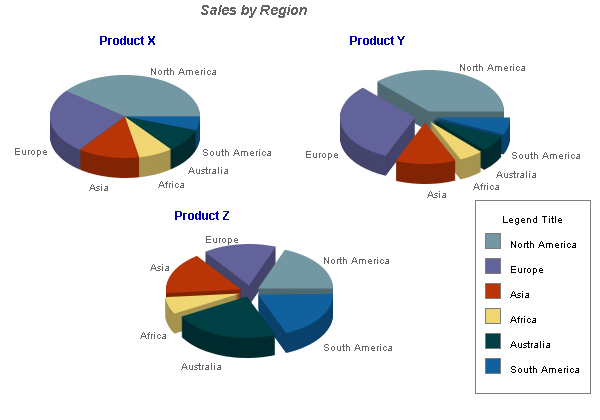
\includegraphics[width=.8\textwidth]{images/servlet3.png}
  \caption[A Pie chart]{Stolen from the net. Google for a pie chart...}
  \label{fig:pie}
\end{figure}

Many graphics packages can produce pdf files
Embedded postscript (file extension .eps) are also a good candidate,
after converting them to pdf with the epstopdf tool. By the way: the
native format of Adobe Illustrator (ai) is similar enough to eps, so
that too can be processed with ps2pdf. Programs like {\em Visual
  Paradigm} are able to produce pdf files too. And sometimes open-office can
lend a helping hand, for by cutting and pasting Windows graphics into
a single page oodraw drawing, you can produce an very usable pdf file. 

Bitmap file types like png and jpeg take up a lot of space in your
final pdf document. 
Bitmap files take even more space if encoded into a pdf file.
If at all possible, stick to a vector format like eps or pdf (if
necessary derived from eps files). 

%\clearpage%to show headers

\section{A png example}
\label{page:pngexample}
If latex cannot fit the diagram on this page
(page~\pageref{page:pngexample}), 
 then you may find the diagram as figure~\vref{fig:pie}. And as you
 can see, you can easily reference pages and images.

%\clearpage%to show headers
\section{PDF from an UML package} 
\label{sec:pdffromuml}
% Note how this varioref expands to
% something like on the next page.
% and using a wrapfigure
\begin{wrapfigure}{r}{.4\textwidth}

  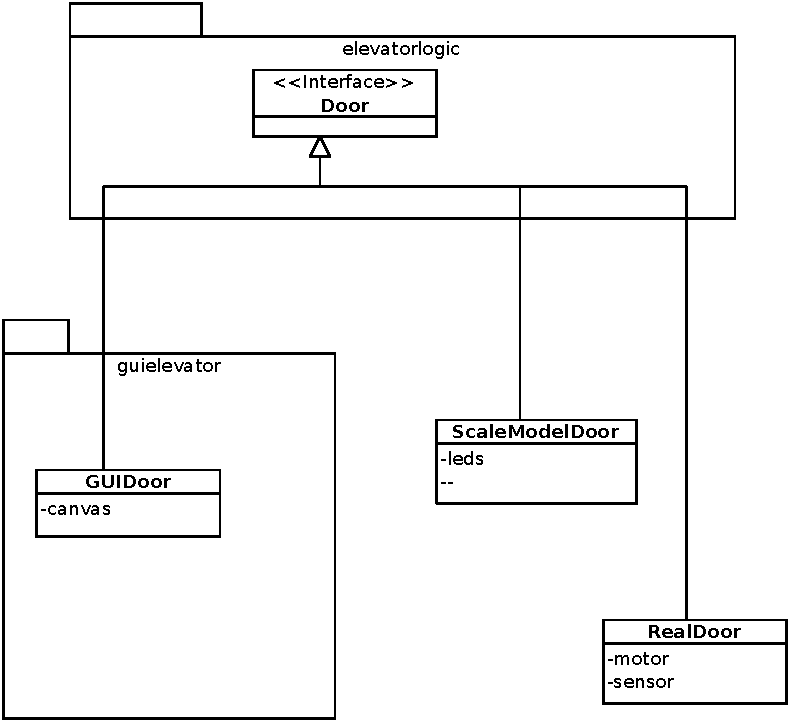
\includegraphics[width=.4\textwidth]{images/doorsystem.pdf}
  \caption{A class diagram made with Visual Paradigm}
  \label{fig:classdiagram}
\end{wrapfigure}
If the documentation you write is a design document of some software
package, you may want to include design diagrams.
No software engineering without a UML diagrams\ldots.
You can see one generated with ``dia'', a vector drawing program that
understands the UML in figure~\ref{fig:classdiagram}
~\vpageref{fig:classdiagram}. This diagram is 'wrapped' in a \Code{wrapfigure} environment, so the text may flow around it

The diagram is not very sophisticated but shows an example of a vector
format file included via an eps$\rightarrow$ pdf conversion by
epstopdf.

Open source programs like umlet, but also commercial ones like Visual Pradigm are also able to produce
vector format graphics files. And sometimes it is helpful to add a box
that is a bit bigger then the picture you want to include.
This ensures that the so called bounding box does not cut of any lines
you want in your picture. Sometimes it is necessary to give these
tools a helping hand with inkscape, that is do a bit of tinkering to
get all details right. Or with \Code{pdfcrop} which typically comes with your \LaTeX installion.

\begin{figure}[htbp]
  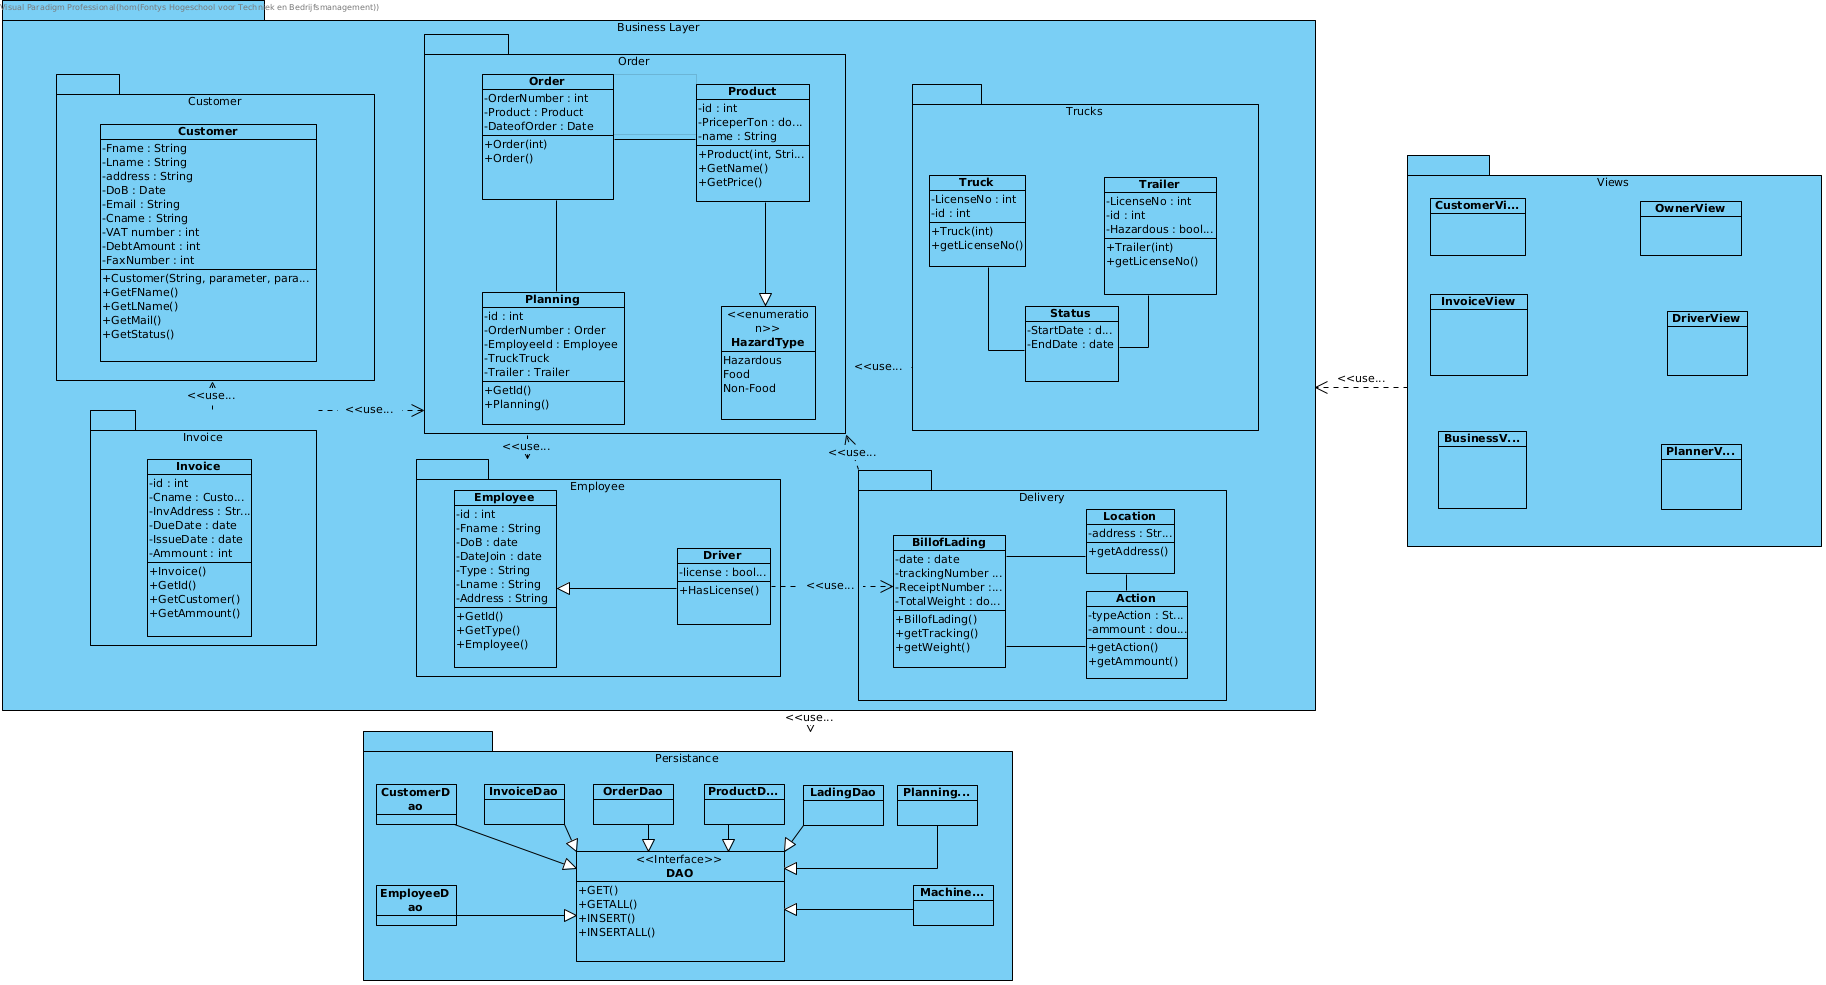
\includegraphics[width=\linewidth]{images/ClassDiagram1.png}
  \caption{You have been warned, NO PNG}
\end{figure}

\begin{wrapfigure}{r}{.4\textwidth}
  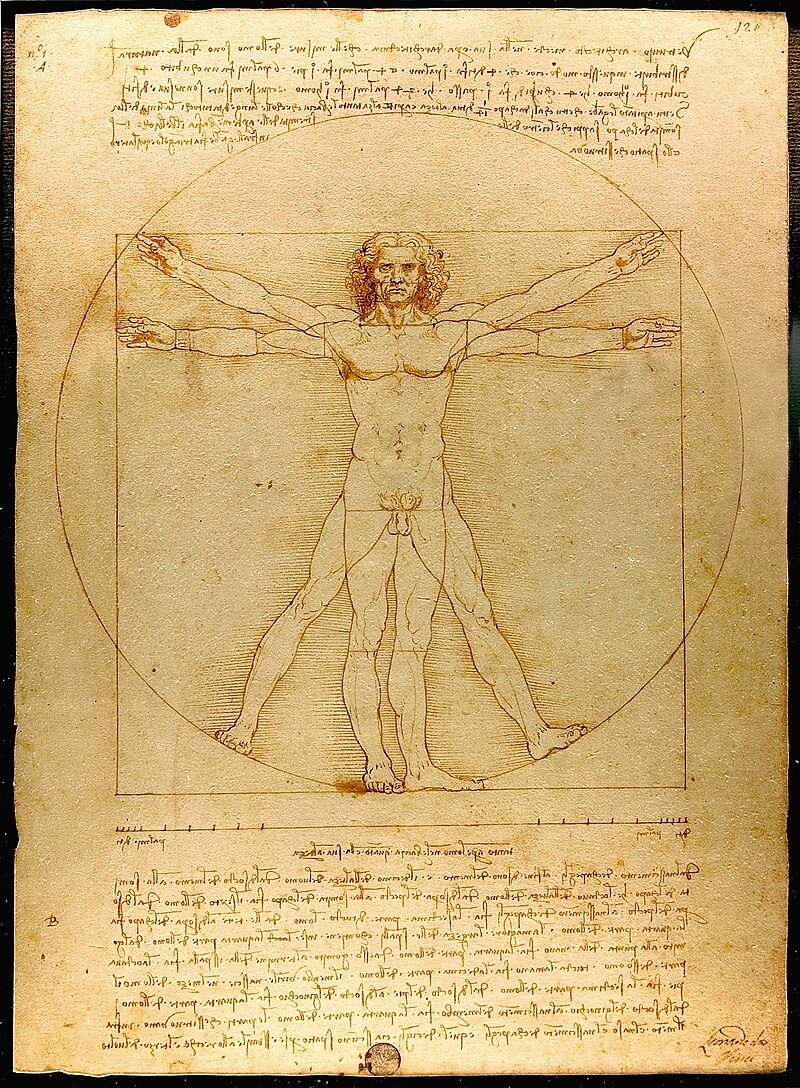
\includegraphics[width=.4\textwidth]{images/Da_Vinci_Vitruve_Luc_Viatour.jpg}
  \caption{Left/right is has, up/down is inheritance}
\end{wrapfigure}
The picture above is wrong on many fronts.
\begin{Itemize}
\item it uses png as image format, where a vector format is provided by the modeling application Visual Paradigm.
  However when you like a pixelated world such as in the game MineCraft, you might feel at home if you zoom in a bit.
\item The arrows point in all directions, which is bad style. A proper UML class diagram should be stylish to improve comprehensibility, as it is recognizable at a glance. Think of Da Vinci's Vitruvian man.
\item It has the VPP blues, that is the colours used are completely non-functional, and also impair readability because the used colour lowers the contract.
\end{Itemize}

Look on the next page how it is done properly.
\clearpage

\begin{figure}[htbp]
  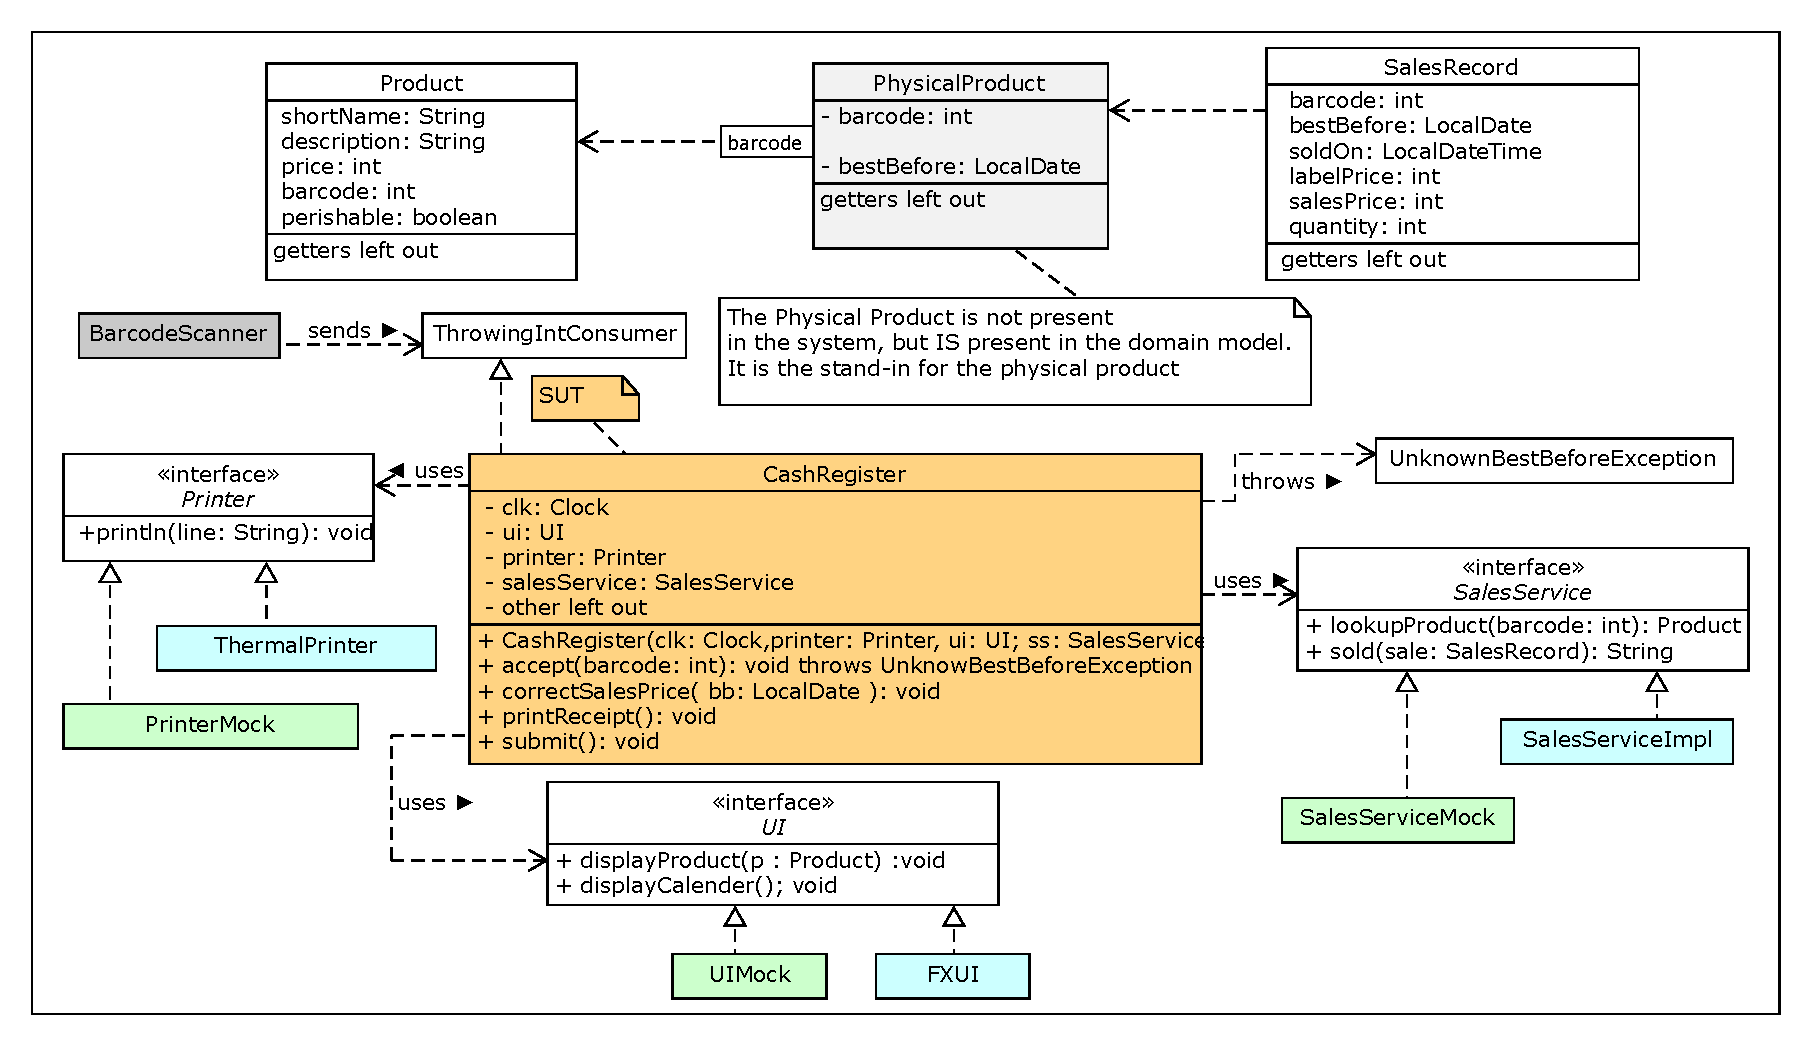
\includegraphics[width=\linewidth]{images/perishablesales.pdf}
  \caption{\label{fig:cashregistertest}Vector format (exported as pdf), with functional colour and a legend}
\end{figure}

\subsection{Stylish UML Class diagram}
\label{sec:stylish}
In the diagram of figure~\vref{fig:cashregistertest} above has style and uses functional colours which are simply explained in a legend.

Good style in a class diagram means:
\begin{Itemize}
\item There is always a direction. Arrows or triangles. They express dependencies.
\item Inheritance in the vertical direction only.
  \begin{Itemize}
    \item Any line that leaves at the top of a class box implies that this
      implements (dashed line) or extends (solid line), without looking where the line ends.
    \item Any triangle that enters at the bottom says that this class is extended or implemented for interfaces.
  \end{Itemize}
  \item All other relationships enter or leave at the left or right edge of the box, so you know things are used
  or this class is used/known.
  \begin{Itemize}
  \item If the local name is relevant, then that name is at the side of the using class, like barcode at the PhysicalProduct which identifies a Product in the system. Internally barcode is a simple number like an \Code{int} or \Code{long}.
  \end{Itemize}
\end{Itemize}

Other than style there are other advantages in this kind of diagrams.
\begin{Itemize}
\item You can zoom in as much as your viewer allows without getting a MineCraft world or worse.
\item A reviewer (the examiner, your coach or someone working with your documents) can select the texts in the diagram and can mark it. You too could do that to embellish the diagram.
\item There is no way that you can do that nicely with a pixel format like png or jpeg.
\end{Itemize}

%%% Local Variables: 
%%% mode: latex
%%% TeX-master: "main"
%%% End: 

\def\TheFile{ch05_codelisting.tex}
\chapter{Listings and Code Documentation}

Just as much as you can have bad style when including diagrams, the same can happen if
you want to show code snippets.

\begin{Itemize}
\item {\color{red!60!black}\Huge{}NEVER} use screenshots from your IDE and even less so, screenshots with a dark theme.
  Typically your report is read on a white background and the contrast with dark themes is really really bad.
\item In the times you had to print your report I would ask the student who soaked the page with black ink.
\item Big diagram tend to produce big files and hence also humongous pdf files.
\end{Itemize}

\begin{figure}
  \caption{Bad, Bad way to show quality code}
  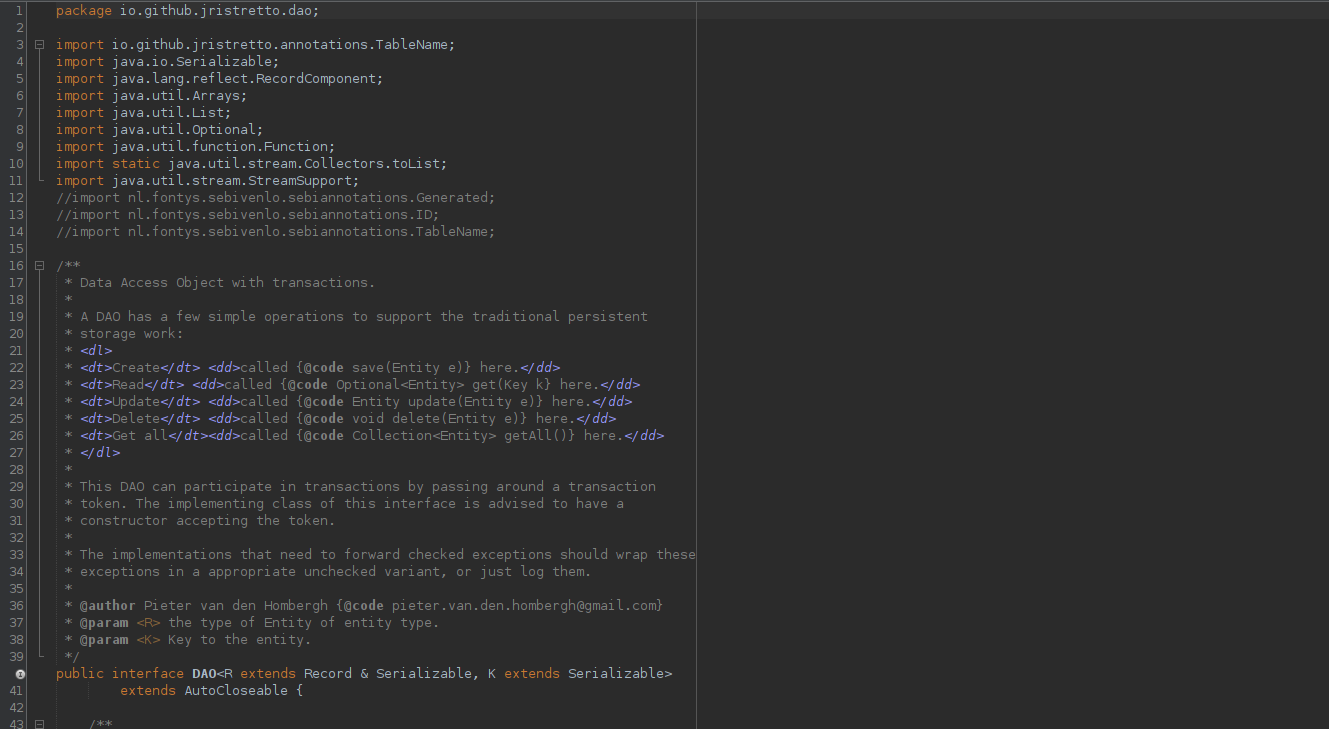
\includegraphics[width=\textwidth]{images/dao.png}
\end{figure}

For these functions to work you need to use the \texttt{package} listings.
See mydefs.tex for the inclusion.

\lstset{%first some settings
  numbers=right, % number the lines
  numberstyle={\tiny\color{red}},frameround=tttt,framerule=1pt,rulesepcolor=\color{gray},
  framexrightmargin=5mm
}

Note that the line numbers in the right hand border are the line
numbers in the included sources.

%% A good advice is to start using \define{doxygen} for your code documentation.
%% It can produce nicely formatted HTML and latex documents and can be
%% tuned in various ways with the  
%% help of doxywizard. The way of working is a lot like using javadoc,
%% but also works for C and C++ files. 
%% See e.g. the documentation on the zthreads package at
%% \url{http://zthread.sourceforge.net} or Qt at 
%% \url{http://doc.trolltech.com/3.3/index.html}

\section{Source code}
The most simple case: include the whole thing with a command like \\
\verb#\lstinputlisting[language=java]{code/Hi.java}#
\lstinputlisting[language=java,caption={Mandatory first program}]{code/Hi.java}

Sometimes it is useful to include just a part of a file, for instance
when you want to explain things. Like what line 11 is all about.\\
\verb#\lstinputlisting[language=java, firstline=11,lastline=11]{Hi.java}#
\lstinputlisting[language=java, firstline=11,firstnumber=11,frame=none,
        lastline=11,numbers=right,basicstyle={\small\ttfamily},
        caption={this is the start of a Java program.}
        ]{code/Hi.java}


The snippet below shows similar code as the snippet in the previous page.
And again, you can zoom in and select text.

\lstinputlisting[language=java, firstline=1,firstnumber=1,
        lastline=39,numbers=right,basicstyle={\tiny\ttfamily},
        caption={The proper way to show your code.}
        ]{code/DAO.java}


%% \section{Makefiles}
%% You can also include make files.
%% Note that makefiles have a peculiar syntax. \define{Spaces and tabs in
%%   Makefiles}\ are meaningful. 
%% That's why I made them show up in the next listing with the command\\
%% \lstinputlisting[firstline=65,lastline=67]{chapters/ch05_codelisting.tex}
%% \lstset{showspaces=true,showtabs=true}
%% Spaces show up as \lstinline| |, tab characters as an extended version
%% of the same thing (\lstinline|	|). 
%% As can be expected, spaces and tabs have no special meaning in
%% makefile comments, the lines starting with a hash (\#) sign. 
%% If you want to know more on makefiles try google or info:make in
%% konqueror on a decently installed Linux box.  

%% The make file for this entire document looks like this:
%% \lstinputlisting[language=make,showtabs=true,
%%      showspaces=true,basicstyle={\ttfamily\scriptsize},
%%      numbers=right,language=make]{Makefile}


%%% Local Variables: 
%%% mode: latex
%%% TeX-master: "main"
%%% End: 

\renewcommand\TheFile{ch06_programmedgraphics.tex}
% \begin{savequote}[15cm]
%   \raggedleft
%  \sffamily
%   A drawing created with just a few words.\\ 
%   Or the old adagium 'a thousand words' reversed.
%   \qauthor{Private experience}
% \end{savequote}
\chapter{Drawing in \LaTeX}

There are quite a few developers who add usefull packages to 
the \TeX world. One of them is Till Tantau of the ``Technische
Üniversität'' in Berlin Germany. He produced the package called pgf,
which stands for portable graphics format. 


The pgf package contains the macro tool \texttt{tikz}, that allows you to draw 
quite nice graphics with just a few commands. Like this small ellipse:
\tikz \draw[rotate=30] (0,-1) ellipse (5pt and 3pt);

The pgf manual has many nice examples that may prove usefull,
certainly if you want to use the package beamer\footnote{also by Till
  Tantau} to create professional looking pdf presentations with \LaTeX.

A simple figure from the pgf manual:

\begin{figure}[htbp]
\begin{tikzpicture}[scale=2,cap=round]
  % Local definitions
  \def\costhirty{0.8660256}

  % Colors
  \colorlet{anglecolor}{green!50!black}
  \colorlet{sincolor}{red}
  \colorlet{tancolor}{orange!80!black}
  \colorlet{coscolor}{blue}

  % Styles
  \tikzstyle{axes}=[]
  \tikzstyle{important line}=[very thick]
  \tikzstyle{information text}=[rounded corners,fill=red!10,inner sep=1ex]

  % The graphic
  \draw[style=help lines,step=0.5cm] (-1.4,-1.4) grid (1.4,1.4);
  
  \draw (0,0) circle (1cm);

  \begin{scope}[style=axes]
    \draw[->] (-1.5,0) -- (1.5,0) node[right] {$x$} coordinate(x axis);
    \draw[->] (0,-1.5) -- (0,1.5) node[above] {$y$} coordinate(y axis);

    \foreach \x/\xtext in {-1, -.5/-\frac{1}{2}, 1}
      \draw[xshift=\x cm] (0pt,1pt) -- (0pt,-1pt) node[below,fill=white] {$\xtext$};
  
    \foreach \y/\ytext in {-1, -.5/-\frac{1}{2}, .5/\frac{1}{2}, 1}
      \draw[yshift=\y cm] (1pt,0pt) -- (-1pt,0pt) node[left,fill=white] {$\ytext$};
  \end{scope}
    
  \filldraw[fill=green!20,draw=anglecolor] (0,0) -- (3mm,0pt) arc(0:30:3mm);
  \draw (15:2mm) node[anglecolor] {$\alpha$};
    
  \draw[style=important line,sincolor]
    (30:1cm) -- node[left=1pt,fill=white] {$\sin \alpha$} (30:1cm |- x axis);
  
  \draw[style=important line,coscolor]
    (30:1cm |- x axis) -- node[below=2pt,fill=white] {$\cos \alpha$} (0,0);
  
  \draw[style=important line,tancolor] (1,0) -- node[right=1pt,fill=white] {
    $\displaystyle \tan \alpha \color{black}=
    \frac{{\color{sincolor}\sin \alpha}}{\color{coscolor}\cos \alpha}$}
    (intersection of 0,0--30:1cm and 1,0--1,1) coordinate (t);

  \draw (0,0) -- (t);
  
  \draw[xshift=1.85cm]
    node[right,text width=6cm,style=information text]
    {
      The {\color{anglecolor} angle $\alpha$} is $30^\circ$ in the
      example ($\pi/6$ in radians). The {\color{sincolor}sine of
        $\alpha$}, which is the height of the red line, is
      \[
      {\color{sincolor} \sin \alpha} = 1/2.
      \]
      By the Theorem of Pythagoras ...
    };
\end{tikzpicture}
\caption[A pgf/Tikz drawing]{A drawing taken from the pgf
  manual/tutorial by Till Tantau}
\label{fig:tikz}
\end{figure}

%%% Local Variables: 
%%% mode: latex
%%% TeX-master: "main"
%%% End: 

\renewcommand\TheFile{ch07_poser.tex}
\begin{savequote}[15cm]
  \vspace{-30mm}
  \raggedleft
  \sffamily
  Never start reading a difficult book at the wrong side.\\ 
  It makes you feel stupid.
  \qauthor{Private experience}
\end{savequote}
\chapter{Starting yourselves?} 

\lstset{numberstyle={\tiny\color{red}},
  basicstyle={\small},numbers=right,
  rulesepcolor=\color{gray},
  showspaces=false,frame=shadowbox}

This document is indeed a bit of a showcase, but there is more to it.
In essence, most documents are mainly texts. 
And those plain texts take mainly typing and not much more.
The minimal, hello world style \LaTeX\ file is not much 
longer\footnote{Counting headers too!} then the C classic.
\lstinputlisting[caption={Hello \LaTeX{} world}]{simple.tex}

And the pictures, well they are made with other packages, and as long
as those can produce a supported format, you can use them. \TeX\ and
\LaTeX\ have an own drawing language, but explaining that would blow
up this space.
There is a lot of documentation available on \TeX\ and \LaTeX\ and I
could recommend some good books on it.
But you need not run off to the nearest book shop. Lots of
documentation is on the Net, just as the \TeX\ program suite itself. 

Look for instance at \url{http://www.ntg.nl} for the Dutch \TeX\ user group
and \url{http://www.dante.de} for the German user group. They are both very 
alive and kicking.

A very good starting point nowadays is \url{http://en.wikibooks.org/wiki/LaTeX/}

\section{My own definitions}
Standard \LaTeX\ output looks a bit dull but are nicely formatted nonetheless.
If you want to make the most of your own style for your own or your
projects documentation, put your style definitions into a separate
file. That way you can keep all definitions of style and \define{macros} in one
spot. This works especially nicely in an multi part document, so
the other files (and authors) can concentrate on content.

You can \define{define} your own macros in \LaTeX. As an example a macro,
\verb#\define#, which I use
to let words stand out at the outer margin. I use it at the first use
of a word or concept in the text, to aid the reader in finding the
definition. Of course this macro could be extended to put the word
into an index. Which makes it a nice exercise.
\clearpage
The macro is defined as follows:
%\lstinputlisting[caption={The macro is defined as follows},frame=shadowbox,firstline=70,lastline=77]{mydefs.tex}
\begin{lstlisting}[caption={The macro is defined as follows},frame=shadowbox]
% This macro '\define' puts the argument in em 
% and in boldface in the margin.
\newcommand{\define}[1]{% 1 argument
  \mbox{}{\textit{#1}}% italics or em
  \marginpar{\raggedright% no adjust
    \bfseries\hspace{0pt}#1}% bold
} % end of macro

\end{lstlisting}

and is used as \verb#\define{new word}#.

Anyway, in modern times you expect to find the examples somewhere convenient, so here you go.
You can find this example in github at \url{https://github.com/homberghp/bachelor_thesis_tips}

%%% Local Variables: 
%%% mode: latex
%%% TeX-master: "main"
%%% End: 

\renewcommand\TheFile{ch08_citingsimple.tex}

\begin{savequote}[15cm]
  \raggedleft
\sffamily
Everything should be made as simple as possible, but not simpler.
\qauthor{Albert Einstein}
\end{savequote}
\chapter{Citing is simple}

Adding proper references and citations to you document can be a real
burden.
Not so in \LaTeX\ where you can use the facilities of a kind ``database''
and many entries available on the web that be added to that database.

This database can be one file, but just as well a set of files, which
you use to organize you bibliography. The files with these data are
called .bib files. 

\section{Bib\LaTeX}
Bibtex is the traditional way of using citations and creating a bibliography, but its
role has all but been taken over by the more modern Bib\LaTeX.
Both are equally simple to use for the most common use. For each reference that you want to use in your report
you should have a definition like below. Look in the \texttt{references.bib} file for more examples.

For instance if your bib contains this entry for \texttt{Nobody}:
\begin{lstlisting}[language=BibTeX]
@misc{ Nobody06,
   author = "Nobody Jr",
   shorthand={Nobody},
   sortname={nobody},
   title = "My Article",
   year = "2006"
}
\end{lstlisting}
\lstset{language=BibTeX}
Then citing Nobody~\parencite{Nobody06} is easy as
pie:\lstinline|\parencite{Nobody06}|

textcite ``\textcite{Nobody06}'', cite \cite{Nobody06}, parencite \parencite{Nobody06}

Then you need to add one compilation step to your normal workflow:

\begin{lstlisting}[language=sh]
$ pdflatex myarticle
$ biber myarticle
$ pdflatex myarticle
$ pdflatex myarticle
\end{lstlisting}

You can of course easily add that to the makefile introduced in an
earlier chapter.

Bibtex is the standard you want to use if preparing an article of a
journal or magazine. The journal typically also prescribes a specific
bibliography style (defined in a .bst file), which is most likely
already define for or by that journal

\subsection{BibLaTeX and Biber}

A bit more modern is biblatex, which has a much simpler definition
format for bst files. The is a separate \textbf{biber} program to do
the processing instead of the bibtex run.
I have used biber in this version of this latex sample. \parencite{biblatexsite}.

\section{What style to choose}

It appears that Fontys Venlo promotes the so called Harvard style, but that has three issues:
\begin{Enumerate}
\item It is not well defined.
\item Finding a reference in the bibliography is not trivial, because the style does not use the label.
  in the bibliography, making it less useable or at least reader friendly.
\item It is NOT what Fontys Venlo uses internally.
\end{Enumerate}


The official 'harvard'-like style that is promoted by the the slides on canvas
produces the bibliography in ~\vref{fig:harvard}, which is actually authoryear.

\begin{figure}
  \shadowbox{\parbox{\linewidth}{
  \centering      
\includegraphics{images/harvardreferences.pdf}}}
  \caption{\label{fig:harvard}No labels that are easily matched with the references in the report text.}
\end{figure}

The style that Fontys uses internally can be emulated with the
settings used in this report and with a bibliography that uses the
fields \texttt{shorthand} and \texttt{shortname} like below
in~\vref{bib:companion} to give the author control on both what is
used in either citation and the bibliography and also the sorting
applied in the bibliography. This provides the best of both worlds.


\begin{lstlisting}[language=BibTeX,caption={\label{bib:companion}Using \texttt{shorthand} for label and \texttt{sortname}for sorting}]
  @BOOK{latexcompanion,
   author = "Frank Mittelbach and Michel Goossens",
   shorthand={Companion, 2004},
   sortname={companion},
   title = "The {\LaTeX }Companion Second Edition",
   publisher = "Addison-Wesley",
   year = 2004
}
\end{lstlisting}

With these addition, and the biblatex configuration in \vref{snip:bibconfig}, you get the more pleasing bibliography in \vref{fig:fontysharvard}
which hase back references as an additional bonus. These will not work in the image above, but do work with this \textcite{latexcompanion} citation.

A screenshot (still ugly, but useful for once) in \vref{fig:activecitation} shows what that looks like in the pdf-viewer \textbf{evince} on a ubuntu box.

\begin{lstlisting}[language=TeX,caption={\label{snip:bibconfig}Using \texttt{shorthand} for label and \texttt{sortname}for sorting}]
%% citation and bibliography style.
%% This style depends on 'sortname' and 'shorthand' fields in the bib file.
%% This gives you control on what is shown in the labels.
%% If you ommit the shorthand, the styles fall back to a numeric label
\usepackage[
backend=biber,
hyperref=true,
backref=true,
]{biblatex}
\DefineBibliographyStrings{english}{
  backrefpage={cited on p.},
  backrefpages={cited on pp.}
}
% end citation bibliography style.
\end{lstlisting}

\begin{figure}
  \shadowbox{\parbox{\linewidth}{
  \centering 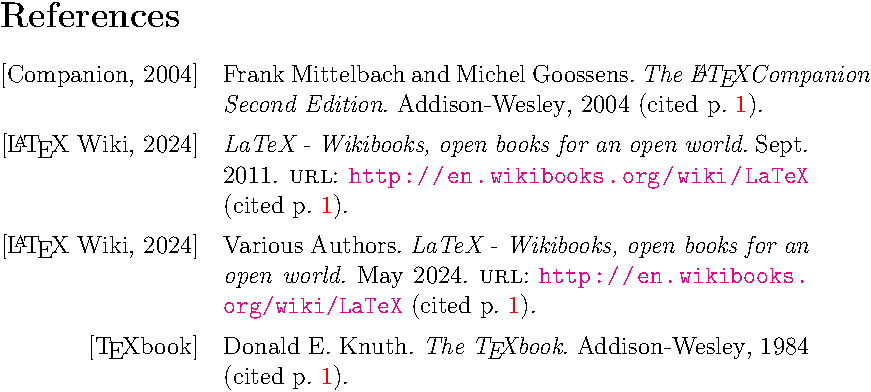
\includegraphics{images/fontysharvard.pdf}}}
  \caption{\label{fig:fontysharvard}Labels same as with the citations.}
\end{figure}


\begin{figure}
   \centering 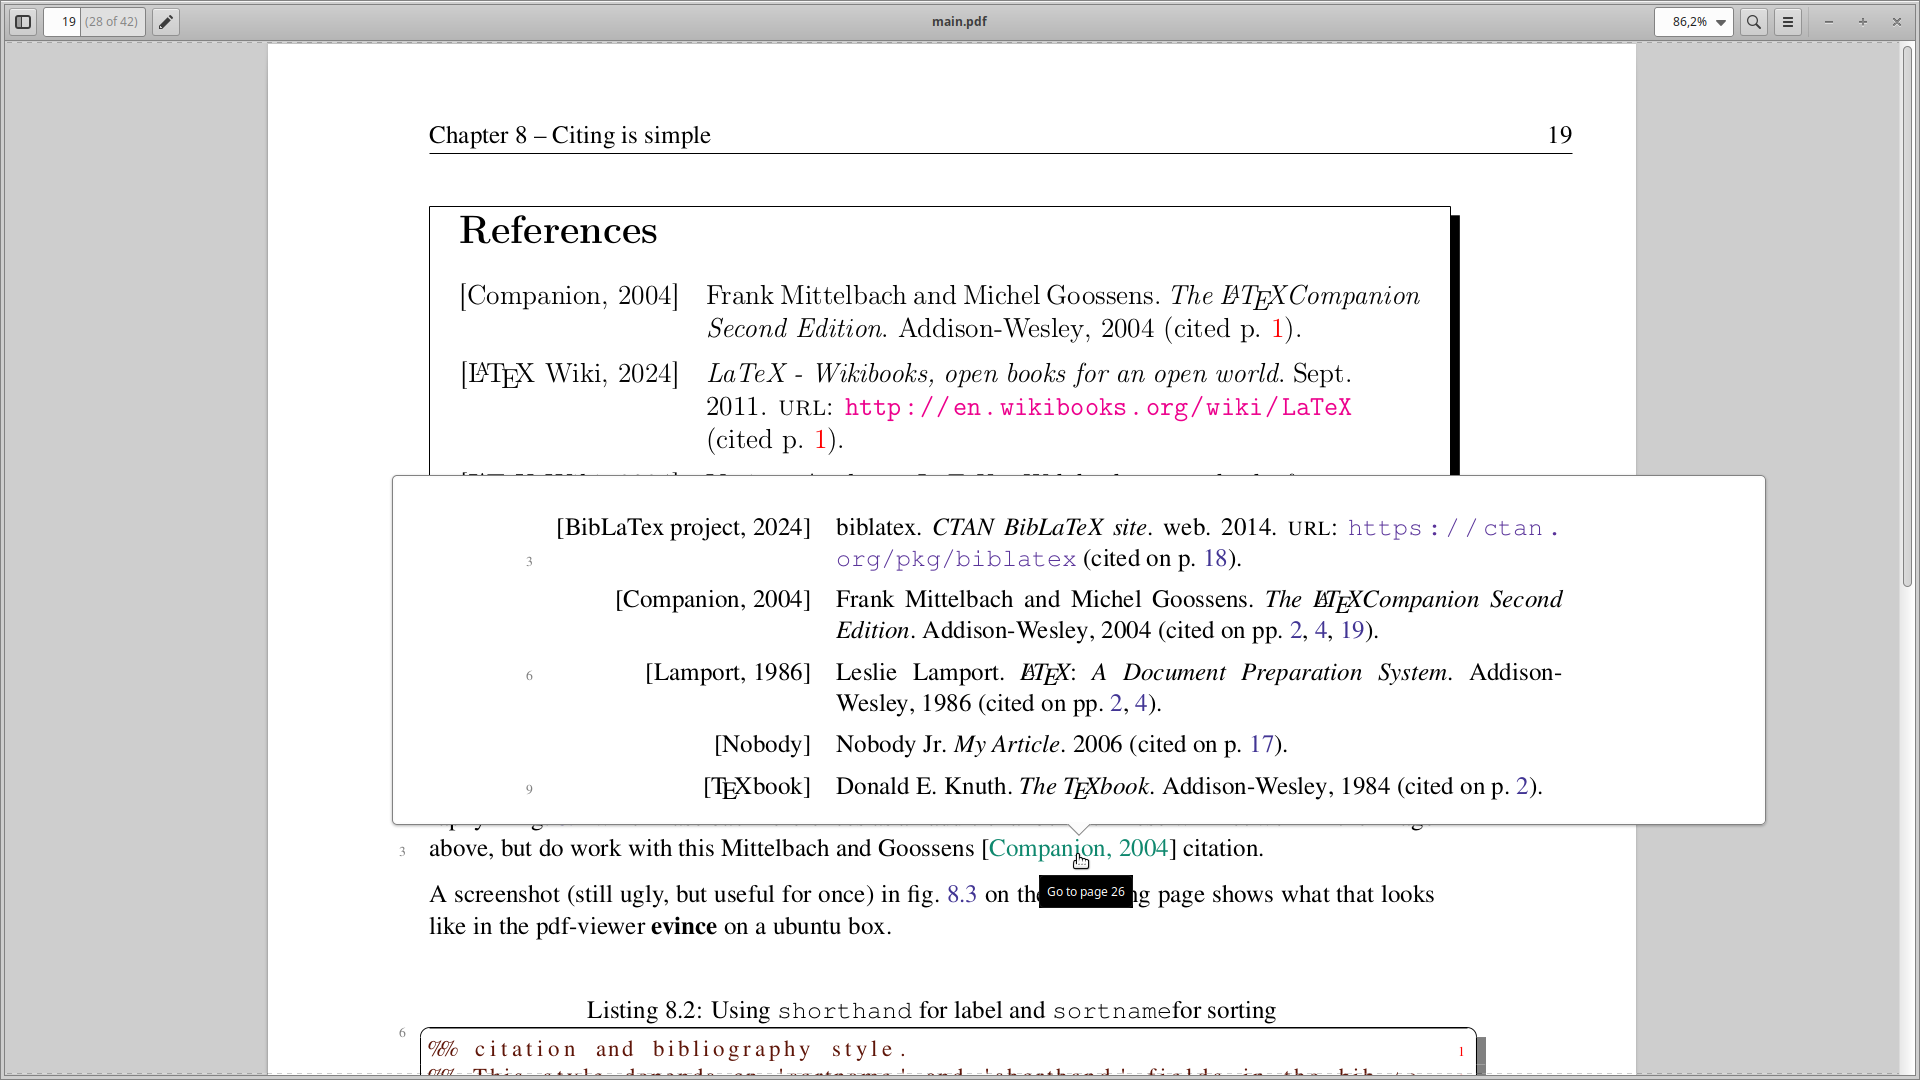
\includegraphics[width=\linewidth]{images/activecitation.png}
  \caption{\label{fig:activecitation}Citations called out when pointed to in evince.}
\end{figure}

As most \LaTeX\ documentation, with a complete installation you can use the command \texttt{texdoc biblatex} to be presented with the
documentaton of \textbf{biblatex} in this example in the default pdf viewer.




\begin{savequote}[15cm]
  \raggedleft
  \sffamily
  Tables, tables, where do I put my tables?
  \qauthor{Anonymous}
\end{savequote}
\chapter{Tables, tables}

Although \LaTeX has its strengths, it is not particularly time effecient when you want to design nice tables.

A spreadsheet (excel, libreoffice calc) may serve you better than having to hand craft tables.

To show what handcrafting can mean you might want to take a look at the sources of the next table.

{
    \setlength{\TabColumnWidth}{24mm}
    \footnotesize\sffamily
    
    \begin{longtable}{| g{.8\TabColumnWidth} | g{\TabColumnWidth} | g{\TabColumnWidth}| g{\TabColumnWidth}| g{\TabColumnWidth}| g{\TabColumnWidth}|}
        \caption{Research results summarized} \label{tab:results}\\
        \hline \rowcolor{Gray}
        \headcell{Criteria} & \headcell{Alt 1} & \headcell{Alt 2} & \headcell{Alt 3} & \headcell{Alt 3} \\\hline
        \endfirsthead
        
        \rowcolor{Gray}
        \multicolumn{5}{l}{{\bfseries \tablename\ \thetable{} Research results summarized -- continued from previous page}} \\\hline
        
        \rowcolor{Gray}
        \headcell{Criteria} & \headcell{Alt 1} & \headcell{Alt 2} &\headcell{Alt 3} & \headcell{Alt 4} \\ \hline
        \endhead
        
        \hline \rowcolor{Gray}\multicolumn{5}{|r|}{{Continued on next page}}\\ \hline
        \endfoot
        
        \hline \hline
        \endlastfoot
        
        % ------ Table content start ------
        \firstcell{.NET 6.0\\Support} & 
        \itemcell{
            \itemC Yes
        } &
        \itemcell{
            \itemC Yes
        } & 
        \itemcell{
            \itemC Yes
            \itemW Since 2022-08-25
        } &
        \itemcell{
            \itemC Yes
        }\\\hline

        
        \firstcell{Documentation} &
        % Traeger
        \itemcell{
            \itemC Online Documentation
            \itemC Examples
        } &
        % softing
        \itemcell{
            \itemC CHM Documentation
            \itemC Examples
            \itemC YouTube Tutorials
        } &
        % UA
        \itemcell{
            \itemC Code Documentation
            \itemC Examples
            \itemC Tutorials
        } &
        % OPC
        \itemcell{
            \itemC GitHub Documentation
        }
        \\\hline

        
        \firstcell{Security} &
        % Traeger
        \itemcell{
            \itemC Signed
            \itemC Sign  \& Encrypt
            \itemC Certificates
        } &
        % softing
        \itemcell{
            \itemC Signed
            \itemC Sign \& Encrypt
            \itemC Certificates
        } &
        % UA
        \itemcell{
            \itemC Signed
            \itemC Sign \& Encrypt
            \itemC Certificates
        } &
        % OPC
        \itemcell{
            \itemC Signed
            \itemC Sign \& Encrypt
            \itemC Certificates
        } \\\hline

        
        \firstcell{License types} &
        % Traeger
        \itemcell{
            \itemC Single Developer License
            \itemC Branch License (=postal address)
        } &
        % softing
        \itemcell{
            \itemC Single Developer License
            \itemX Branch License
        } &
        % UA
        \itemcell{
            \itemC Single Developer License
            \itemX Branch License
        } &
        % OPC
        \itemcell{
            \itemC Branch License
        } \\\hline

        
        \firstcell{Support} &
        % Traeger
        \itemcell{
            \itemC inc. 12 months  Top Level Support
            \itemC Support and  update renewal 12  months (price  depending on  license)
        } &
        % softing
        \itemcell{
            \itemC Dedicated  support team
            \itemW Support is valid  for 3 years and can be extended in 1-year steps afterward
        } &
        % UA
        \itemcell{
            \itemC Includes first-year maintenance  package
            \itemW Includes only  15 support  incidents
        } &
        % OPC
        \itemcell{
            \itemC No support  nor guarantees
        } \\\hline

        
        \firstcell{License} &
        % Traeger
        \itemcell{
            \itemC Unlimited  license lifetime
            \itemC No royalty fees
        } &
        % softing
        \itemcell{
            \itemC All Software  updates included
            \itemC Unlimited runtime  of the \acrshort{sdk} past  of maintenance  contract
            \itemC No royalty fees
            \itemC Available in  source code and  binary
        } &
        % UA
        \itemcell{
            \itemC Includes one  UaModeler license
            \itemC Includes one  UaExpert license
        } &
        % OPC
        \itemcell{
            \itemC OPC Foundation  license
            \itemC Open source
        } \\\hline

        
        \firstcell{Price\\}\footnote{\label{footnote:vat}VAT excluded} &
        % Traeger
        \itemcell{
            \itemC Single developer  license\\Client: \hfill{}990€\\Server: \hfill{}2.175€\\Combined:\hfill{}2.600€
            \itemC Branch license\\Client: \hfill{}2.000€\\Server: \hfill{}4.350€\\Combined:\hfill{}5.200€
        } &
        % softing
        \itemcell{
            \itemC Single developer  license\\Client: \hfill{}3.150€\\Server: \hfill{}6.150€\\Combined:\hfill{}9.662€
        } &
        % UA
        \itemcell{
            \itemC Single seat  developer license\\Combined:\\\hfill{}4.900€
            \itemW Further support costs yearly:\\\hfill{}1.470€
        } &
        % OPC
        \itemcell{
            \itemC Free
        } \\\hline

        
        \firstcell{Costs for 5 yrs} \cref{footnote:vat}\footnote{with no prior license} &
        % Traeger
        \itemcell{
            \itemC 8.320€
            \itemC Unlimited  developers
        } &
        % softing
        \itemcell{
            \itemC 15.862€
            \itemC One developer
        } &
        % UA
        \itemcell{
            \itemW 10.780€
            \itemC One developer
        } &
        % OPC
        \itemcell{
            \itemC 0€
            \itemC Unlimited  developers
        } \\\hline

        
        \firstcell{Other} &
        % Traeger
        \itemcell{
            \itemC Branch license  (Client \& Server)  already bought
            \itemW Further support  costs yearly 780€
        } &
        % softing
        \itemcell{
            \itemC Integrated log  system
        } &
        % UA
        \itemcell{
            \itemW May not be stable  on .NET 6.0
        } &
        % OPC
        \itemcell{
            \itemC Limited features
        } \\\hline

        
        \firstcell{Weblink} &
        % Traeger
        \itemcell{
            \itemU \href{https://www.fontys.nl}{Fontys Home}
        } &
        % softing
        \itemcell{
            \itemU \href{https://github.com/homberghp/bachelor_thesis_tips}{This document}
        } &
        % UA
        \itemcell{
            \itemU \href{https://www.unified-automation.com/products/server-sdk/net-ua-server-sdk.html}{UA~Bundle}
        } &
        % OPC
        \itemcell{
            \itemU \href{https://github.com/OPCFoundation/UA-.NETStandard}{OPC~Foundation General}
        }\\
    \end{longtable}
}


\section{The easy way or the high way}

Luckily, spreadsheets can also create good looking tables. That is their bread and butter right?
And of course, what applies to diagrams and codelistings applies here too. We want to be able to zoom in to any depth
of our liking without landing in the world of MineCraft, so export from the spreadsheet using svg(and convert to pdf) or pdf directly. That way you can have the reviewer zoom in and select text to make his/her remarks.

Here are some examples.

\begin{table}
  \caption{We commonly put table captions at the top}
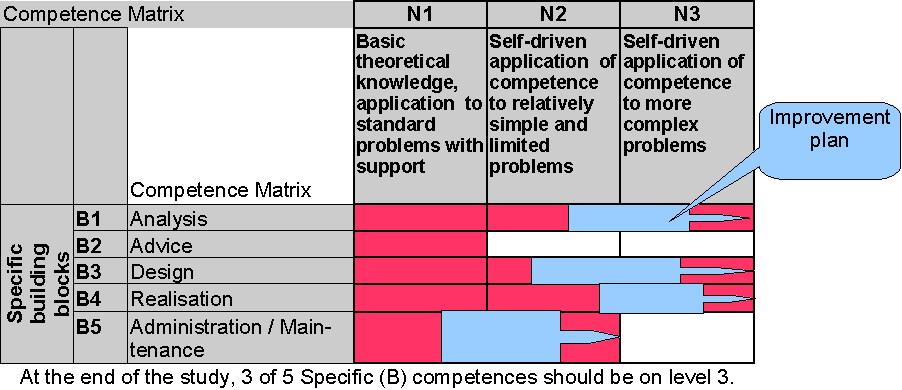
\includegraphics{tables/matrixExample-crop.pdf}   
\end{table}

Note that the \textit{enviroment} is table, but we include the table as if it were an image with includegraphics.

\begin{table}
  \caption{Another table, this time made with word, but included as pdf!}
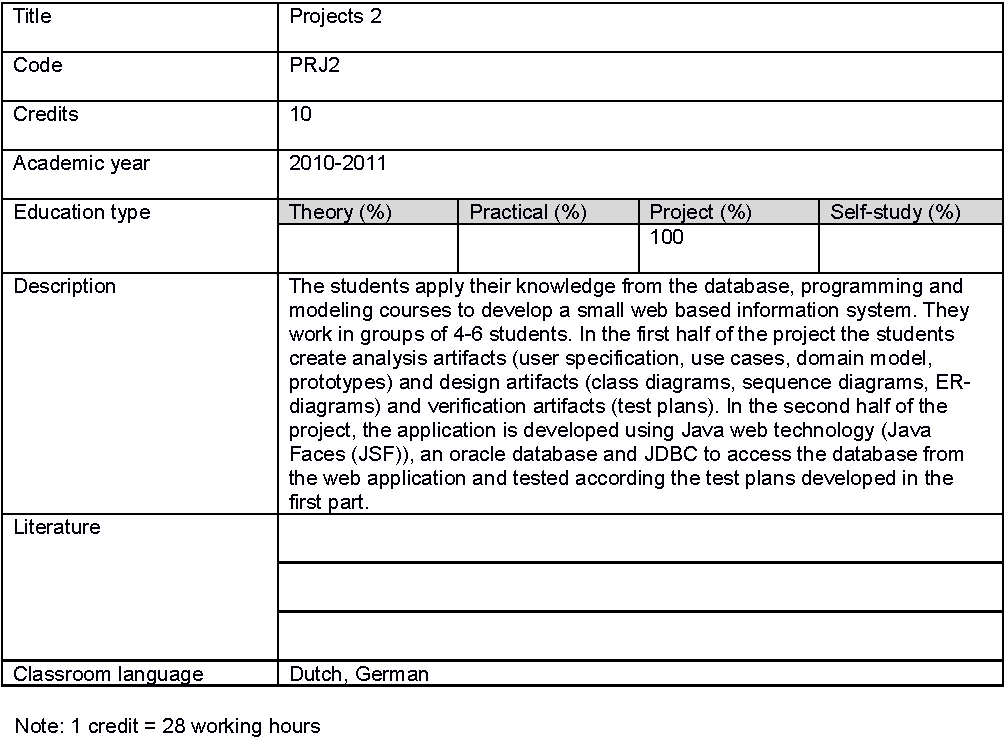
\includegraphics{tables/md_prj2-crop.pdf}   
\end{table}

\begin{table}
  \caption{ESD, still going strong?}
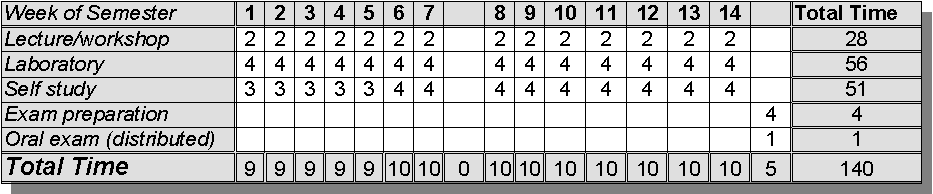
\includegraphics{tables/timetable-crop.pdf}
\end{table}


To prepare the tables, export or print \textit{a selection} of the spreadsheet to pdf without header and footer.
Then use pdfcrop, part of TeXLive, to crop the pdf to just the content. With cropping you remove the white space around the table, so it becomes its true size and appearance.

You can embellish the table in the spreadsheet as much as you like. The fruit of that work will then be visible in is appearance in you report.

All the above works for charts created with a spreadsheet too.

\begin{figure}
  \centering
\shadowbox{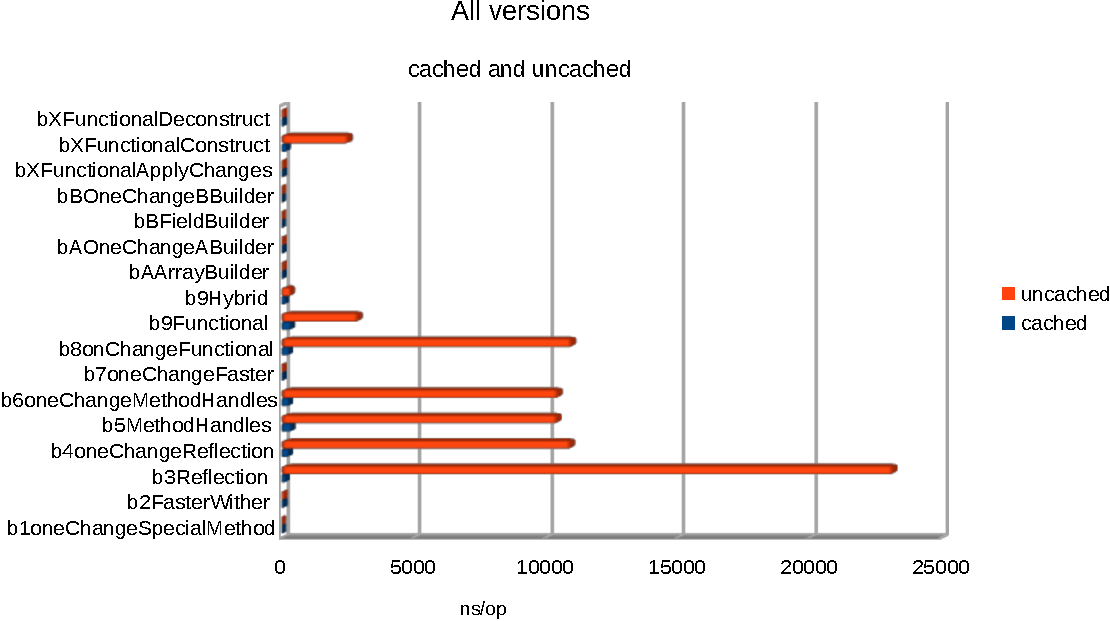
\includegraphics[width=.7\linewidth]{images/all-benchmarks-crop.pdf}}
  \caption{Benchmark results, LibreOffice calc, cropped}
\end{figure}



\begin{savequote}[15cm]
  \raggedleft
\sffamily
The errors you made and are about to make have been made by my said the experienced man to the newby, selling it as wisdom.
\qauthor{You, in the future}
\end{savequote}

\chapter{Tips and Tricks}

\begin{itemize}
\item Either install Latex on your own machine, maybe in a docker-image, or use overleaf. \\
    On your own machine, the compilation will commence more quickly. There is also no compilation timeout, which you may run into with overleaf.
\item actively use $\backslash$include (for chapters) and $\backslash$input to break you 
 big document into smaller parts. If you then have a file called IncludeOnly.tex in your root dir, only the chapters in that file will be included. In this way it is easy to make something for your reviewers, but also speeds up the compilation process drastically, which is nice while you are editing and you work (re)view-driven.
\item If you add pictures or tables, always choose vector format. Never jpeg unless it is a photo, png only for screenshots, which you should try to avoid. In the drawing tool (Visual Paradigm, Umlet, drawio)  you can most likely export in pdf format which you can include with $\backslash$includegraphics. If you have svg, which the other popular vector format, you can use a conversion tool to turn it into a pdf. Inkscape, which is available on all relevant platforms, does the trick for me.
  For tables, a spreadsheet(excel libreoffice calc) is a reasonable choice. Export the selection as pdf with no borders.  Use a tool to clip/crop off the white borders. pdfcrop works for me there. Include the pdf with $\backslash$includegraphics, but put in in table environment.
  
\end{itemize}

%% supress post file when not required
%% \IfFileExists{IncludeOnly.tex}{}{%

% Add the bibliography at the end
\addcontentsline{toc}{chapter}{References}
\printbibliography[title={References}]

% Add appendix
\begin{appendices}
\thispagestyle{empty}
    \renewcommand*{\thepage}{\thechapter-\arabic{page}}%
%% use appendix id + and number as page number.
\pretocmd{\chapter}{%
    \clearpage%
    \renewcommand*{\thepage}{\thechapter-\arabic{page}}%
  }{}{}
  % reset page numbers for appendix
  \pagenumbering{arabic}
  \chapter{Some macro examples}

The first macro defines a new environment.
An environment is something with $\backslash$begin\{environmentname\} and $\backslash$end\{environmentname\}, like an itemize list.
I wanted to tweak the standard lengths that are used, because I found the defaults a bit too spacy.

\begin{lstlisting}[caption={Tighter itemize}]
\newenvironment{Itemize} {
  \begin{itemize}{}% start of envionment with all the settings
    \setlength\topsep{0ex}%
    \setlength\parskip{0ex}%
    \setlength\partopsep{0em}%
    \setlength\parsep{0em}%
    \setlength\itemsep{0em}%
  }{\end{itemize}% end of the environmet
}
\end{lstlisting}


  \pagenumbering{arabic}
  \chapter{Include Listings}

The listing in \vref{lst:proper} was included with this code

\begin{lstlisting}
\lstset{%first some settings
  numbers=right, % number the lines
  numberstyle={\tiny\color{gray}},frameround=tttt,framerule=1pt,rulesepcolor=\color{gray},
  framexrightmargin=5mm
}
\end{lstlisting}

followed by

\begin{lstlisting}
  \lstinputlisting[language=java, firstline=1,firstnumber=1,
  lastline=39,numbers=right,basicstyle={\tiny\ttfamily},
  caption={The proper way to show your code.}
  ]{code/DAO.java}
\end{lstlisting}
      
  \pagenumbering{arabic}
  \chapter{Include using pdfpages}
Include the whole pdf with all pages and some scale down to have our own page numbering.
The pdf has been created from a website using the ``print to pdf'' feature of the \textbf{firefox} web browser which by the way has a very nice pdf viewer with annotation features.
\lstset{language=[LaTeX]TeX}
\begin{lstlisting}[caption={code to include next pages as pdf}]
 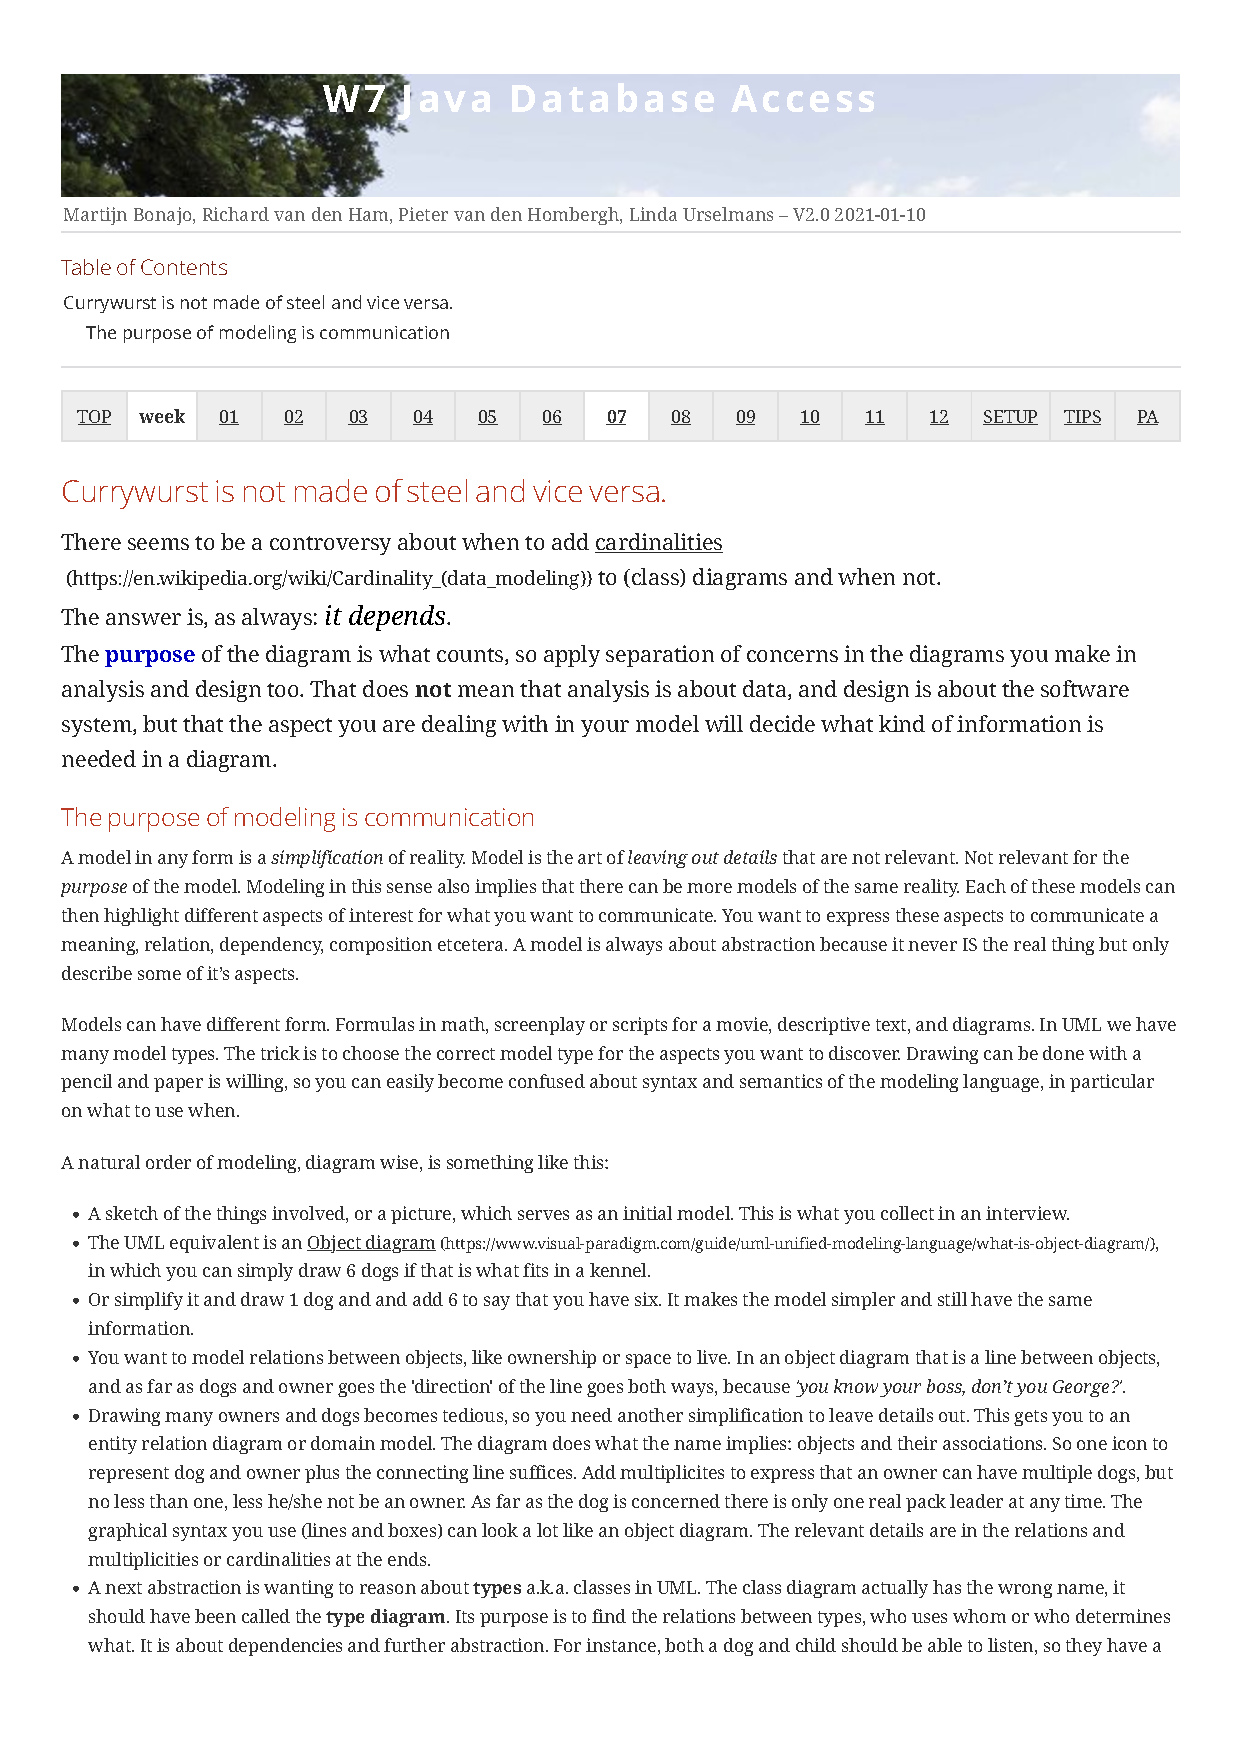
\includepdf[scale=0.9,pages=-,pagecommand={\pagestyle{fancy}}]{appendix/sausageisnotsteel.pdf}
\end{lstlisting}

If you make the documents intended for the appendix in \LaTeX\ too, you should of course simply $\backslash$include them in your report, as all but the last appendix here have been done.
% \pagestyle{empty}
%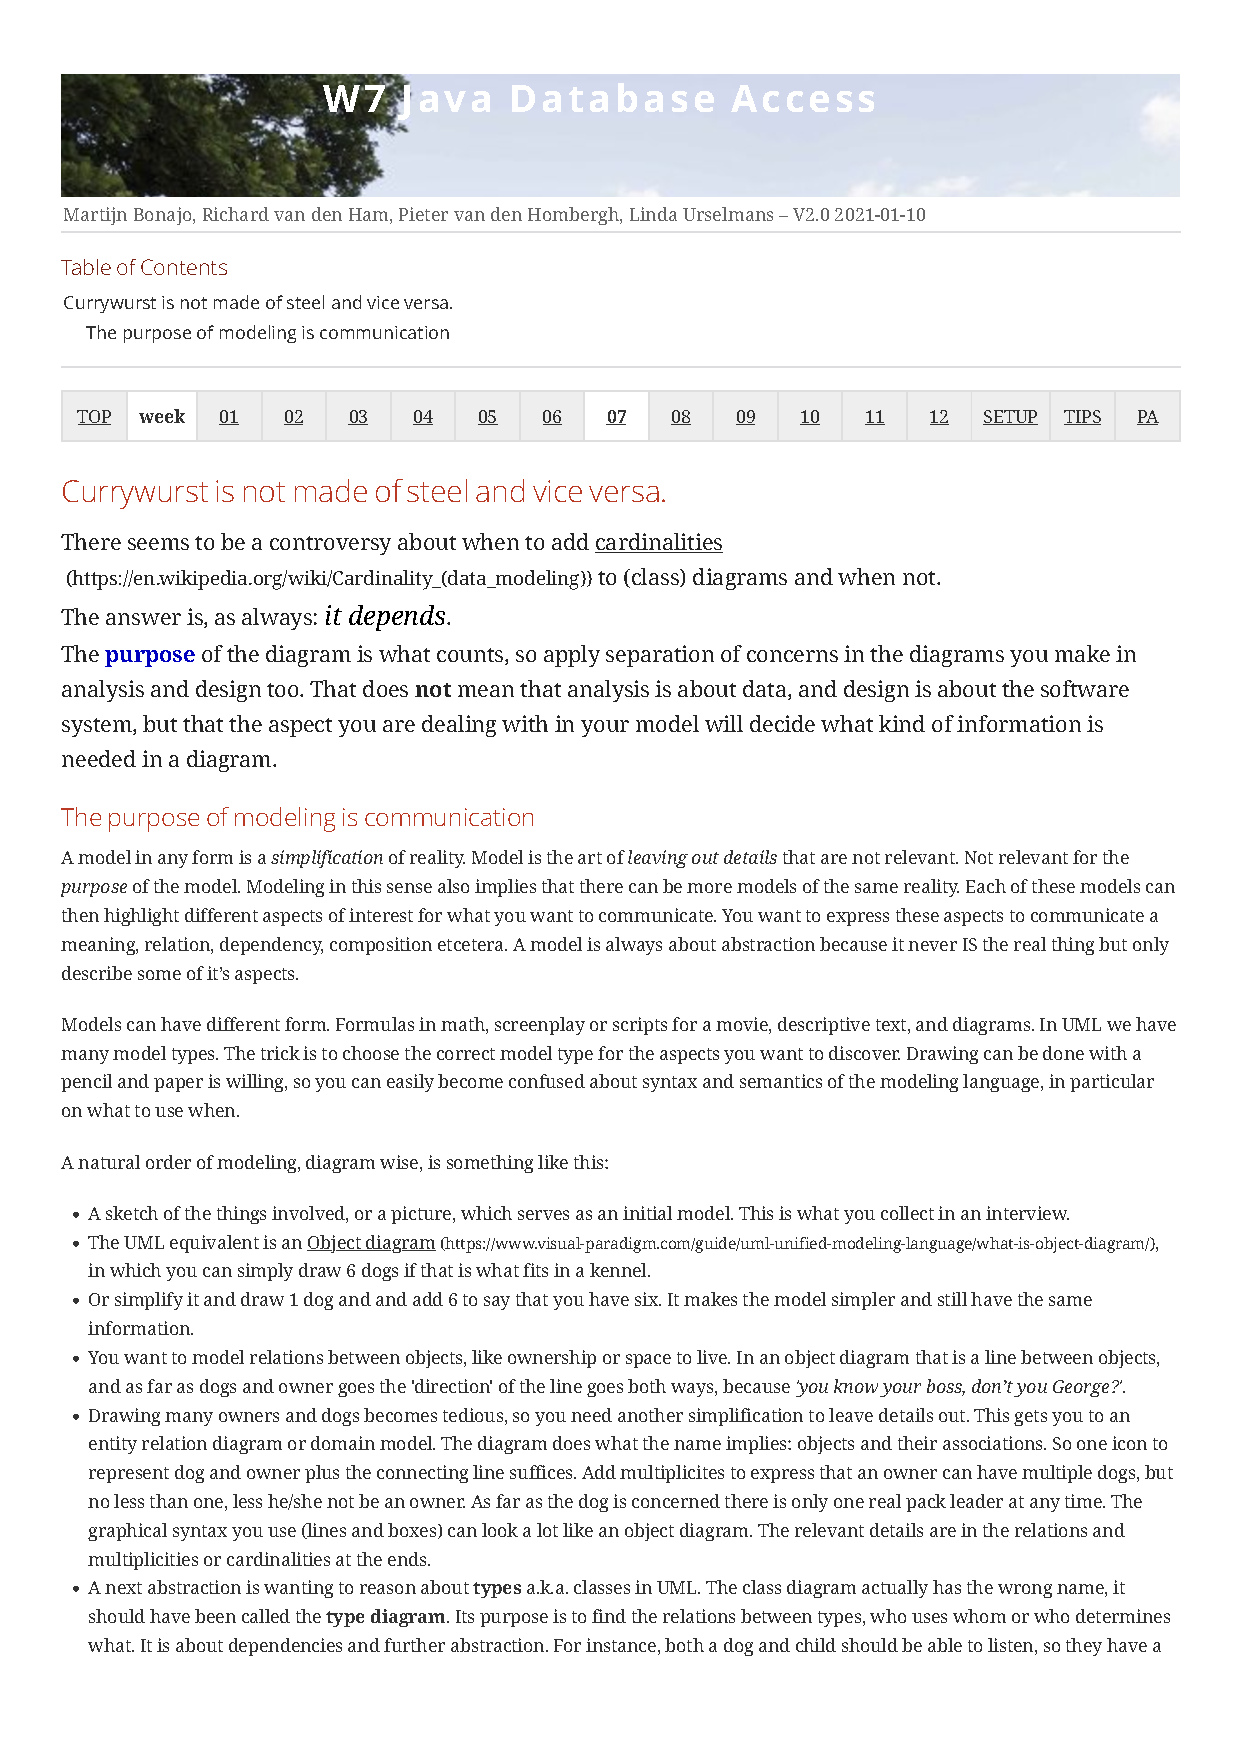
\includepdf[scale=0.9,pages=-,pagecommand={\pagestyle{fancy}}]{appendix/sausageisnotsteel.pdf}
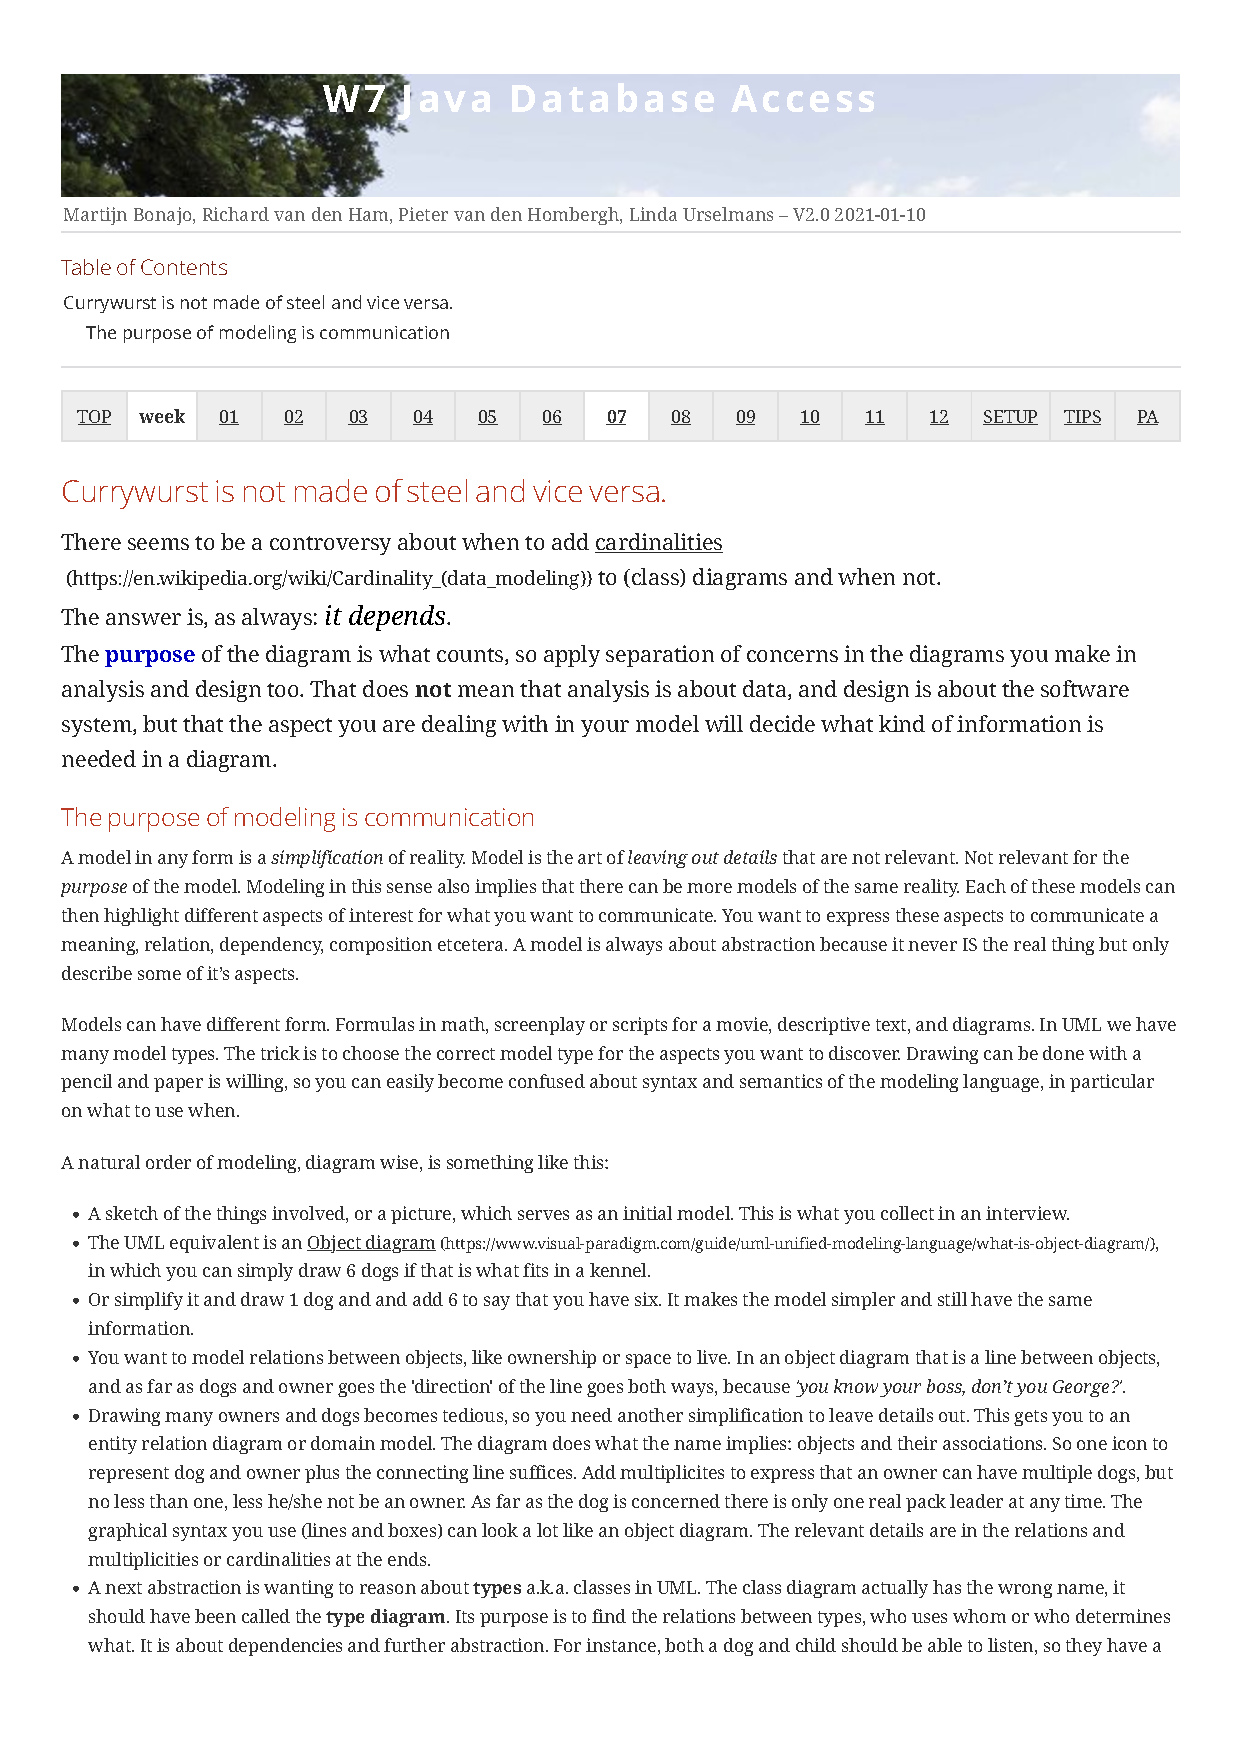
\includepdf[scale=0.9,pages=-,pagecommand={\thispagestyle{appendix}}]{appendix/sausageisnotsteel.pdf}


  \pagenumbering{arabic}
  \chapter{Counting words}

It is mandatory to include the word count of your thesis in the
information page. There are many constructs shown on the Internet but
we choose to go for the simplest solution possible.

\section{What to count}
It is resonable to only count the words in the report proper.
This implies only counting the words in the chapters, which is easy
enough by using the \texttt{texcount} command with a \define{\gls{glob}} for the
chapters: \texttt{chapters/*.tex}

\section{How to count}
\begin{lstlisting}[language=sh]
texcount  -inc -sum  -1 chapters/*.tex > wordcount.txt
\end{lstlisting}

\section{When to count}
To make sure that the word count in the file is updated in the
whenever a chapter file changes, we use the Makefile.

In the Makefile we make the \texttt{wordcount.txt} file dependent on the
chapter files with this simple rule:

\begin{lstlisting}[language=make,showtabs]
wordcount.txt: chapters/*.tex
	texcount  -inc -sum  -1 chapters/*.tex > wordcount.txt
\end{lstlisting}

and make the main.pdf file dependent on the \texttt{wordcount.txt} file as
well.

When that does not work for you, maybe, because you cannot or will not
use \texttt{make} in your environment, then execute the
\texttt{texcount} as given above in the terminal.

Even simpler, delete the \texttt{wordcount.txt} file and run pdflatex
again.


\end{appendices}

%}
\end{document}
